
\documentclass[compress]{beamer}

%\usepackage{beamerthemesplit}
\usepackage{xmpmulti}

\usepackage{booktabs}
\usepackage{graphicx,float,wrapfig, bbm}
\usepackage{amsfonts, bbold, comment}
\usepackage{mdwlist}
\usepackage{subfigure}
\usepackage{colortbl}
\usepackage{overpic}
\usepackage{pdfpages}

\usepackage{multirow}

\pgfdeclareimage[width=\paperwidth]{mybackground}{../../common/boulder.pdf}

\newcommand{\slda}[0]{\abr{slda}}
\newcommand{\bm}[1]{\mbox{\boldmath$#1$}}
\newcommand{\lda}[0]{\abr{lda}}
\newcommand{\explain}[2]{\underbrace{#2}_{\mbox{\footnotesize{#1}}}}
\newcommand{\itmspace}[0]{\hspace{2cm}}
\newcommand{\pos}[1]{{\texttt{#1}}}
\newcommand{\e}[2]{\mathbb{E}_{#1}\left[ #2 \right] }
\newcommand{\ind}[1]{\mathbb{I}\left[ #1 \right] }
\newcommand{\abr}[1]{\textsc{#1} }
\newcommand{\ex}[1]{\mbox{exp}\left\{ #1\right\} }
\newcommand{\g}{\, | \,}
\newcommand{\citename}[1]{#1 }
\newcommand{\fsi}[2]{
\begin{frame}[plain]
\vspace*{-1pt}
\makebox[\linewidth]{\includegraphics[width=\paperwidth]{#1}}
\begin{center}
#2
\end{center}
\end{frame}
}


\newcommand{\danquote}[1]{

\begin{flushright}
\begin{overpic}[width=5.5cm,tics=10]{general_figures/speech_bubble}
	\put(10,30) { \parbox{4cm}{#1 }}
\end{overpic}

\includegraphics[width=1.5cm]{general_figures/milkman_dan}
\end{flushright}
}


\newcommand{\gfxi}[2]{
\begin{center}
	\includegraphics[width=#2\linewidth]{interpretability/#1}
\end{center}
}

\newcommand{\gfxs}[2]{
\begin{center}
	\includegraphics[width=#2\linewidth]{simtrans/#1}
\end{center}
}

\newcommand{\gfxq}[2]{
\begin{center}
	\includegraphics[width=#2\linewidth]{qb/#1}
\end{center}
}


\newif\ifjobtalk\jobtalktrue
\newif\iflong\longtrue

\usetheme[
          showdate=true,                     % show the date on the title page
          alternativetitlepage=true,         % Use the fancy title page.
          titlepagelogo=general_figures/shell,              % Logo for the fir\
st page.
          ]{UMD}


\title[]{If You Want Interpretable AI, Measure It}
\author{ Jordan Boyd-Graber}
\date{2022}

\institute[] % (optional, but mostly needed)
{University of Maryland}


%gets rid of bottom navigation symbols
\setbeamertemplate{navigation symbols}{}

%gets rid of footer
%will override 'frame number' instruction above
%comment out to revert to previous/default definitions
\setbeamertemplate{footline}{}

\begin{document}

\frame{
\titlepage
\tiny
}

\begin{frame}[plain]
\vspace*{-1pt}
\only<1>{\makebox[\linewidth]{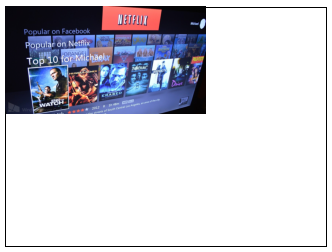
\includegraphics[width=\paperwidth]{general_figures/ml_intro_1}}}
\only<2>{\makebox[\linewidth]{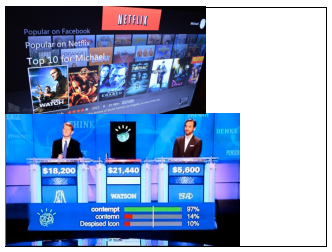
\includegraphics[width=\paperwidth]{general_figures/ml_intro_2}}}
\only<3>{\makebox[\linewidth]{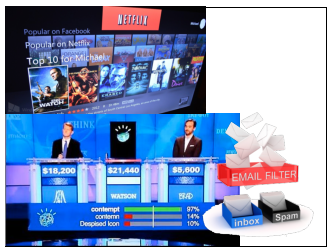
\includegraphics[width=\paperwidth]{general_figures/ml_intro_3}}}
\only<4>{\makebox[\linewidth]{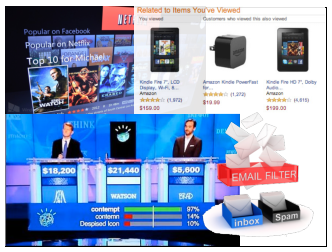
\includegraphics[width=\paperwidth]{general_figures/ml_intro_4}}}
\only<5>{\makebox[\linewidth]{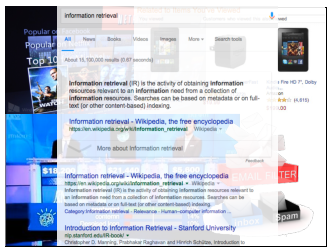
\includegraphics[width=\paperwidth]{general_figures/ml_intro_5}}}
\only<6->{\makebox[\linewidth]{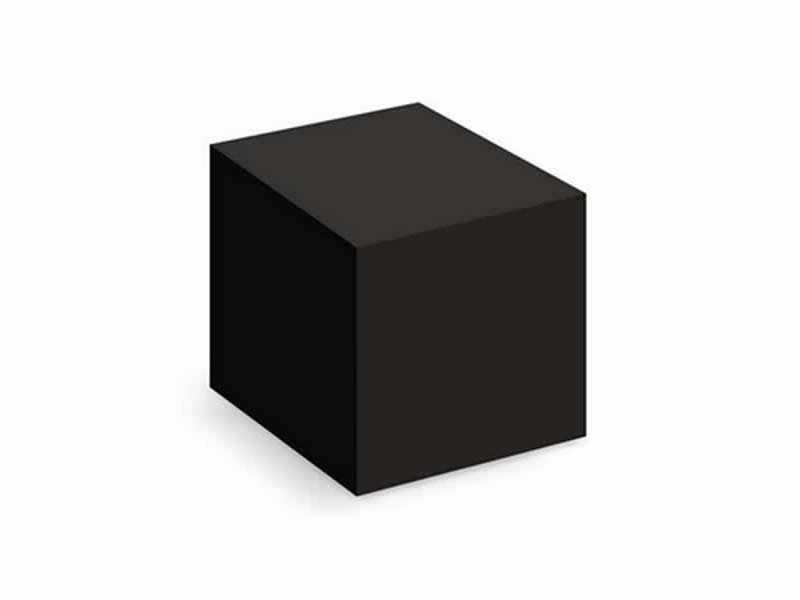
\includegraphics[width=\paperwidth]{general_figures/blackbox}}}
\only<7>{

\vspace{-5cm}
\begin{block}{Outline}
  \begin{itemize}
  \item AI should be interpretable
    \item We should measure interpretability    
  \item Proposal for Unsupervised Methods (Topic Models)
    \item Proposal for Supervised Methods (Question Answering / Translation)
  \end{itemize}
\end{block}

}
\end{frame}


\begin{frame}
\frametitle{The Challenge of Big Data}

\begin{columns}

\column{.5\linewidth}

Every second \dots
\begin{itemize}
  \item 600 new blog posts appear
  \item 34,000 tweets are tweeted
  \item 30 GB of data uploaded to Facebook
\end{itemize}
\pause

\begin{block}{Unstructured}
  No XML, no semantic web, no annotation.  Often just raw text.
\end{block}

\column{.5\linewidth}

\only<3->{
Common task: what's going on in this dataset.
\begin{itemize}
   \item Intelligence analysts
   \item Brand monitoring
   \item Journalists
   \item Humanists
\end{itemize}
}
\only<4>{
\centering
Common solution: unsupervised machine learning (topic models)
}

\end{columns}

\end{frame}

\begin{frame}

\begin{center}
\frametitle{What does a Topic Model do?}
From an \textbf<1>{input corpus} and number of topics \textbf<1>{$K$} $\rightarrow$ \textbf<2>{words to topics} \\
\only<1>{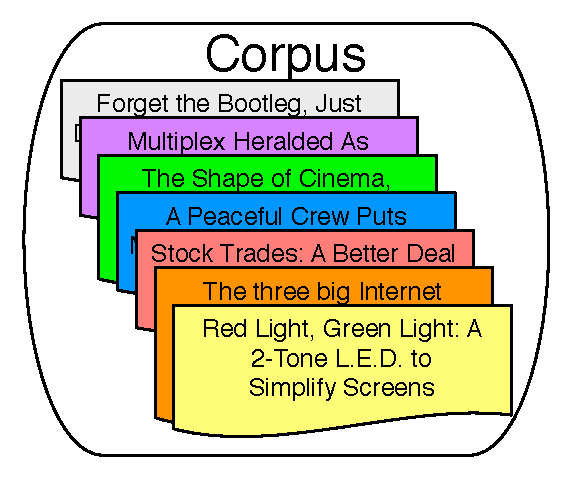
\includegraphics[width=0.6\linewidth]{reading_tea_leaves/figures/heldout_0} }
\only<2>{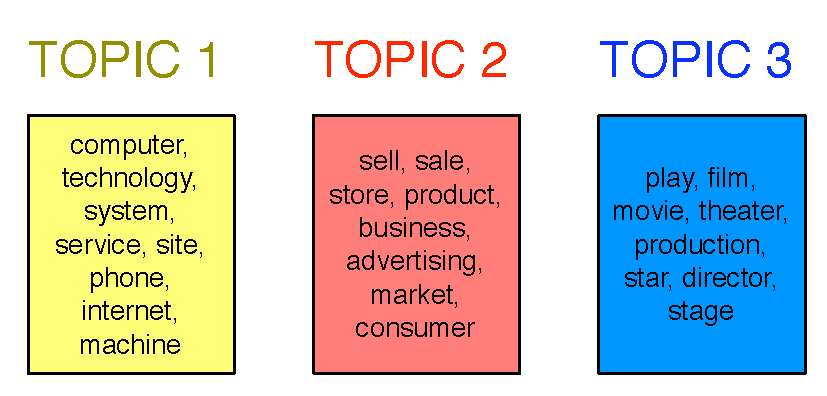
\includegraphics[width=0.9\linewidth]{reading_tea_leaves/figures/nyt_topics_wide}}
%\only<3>{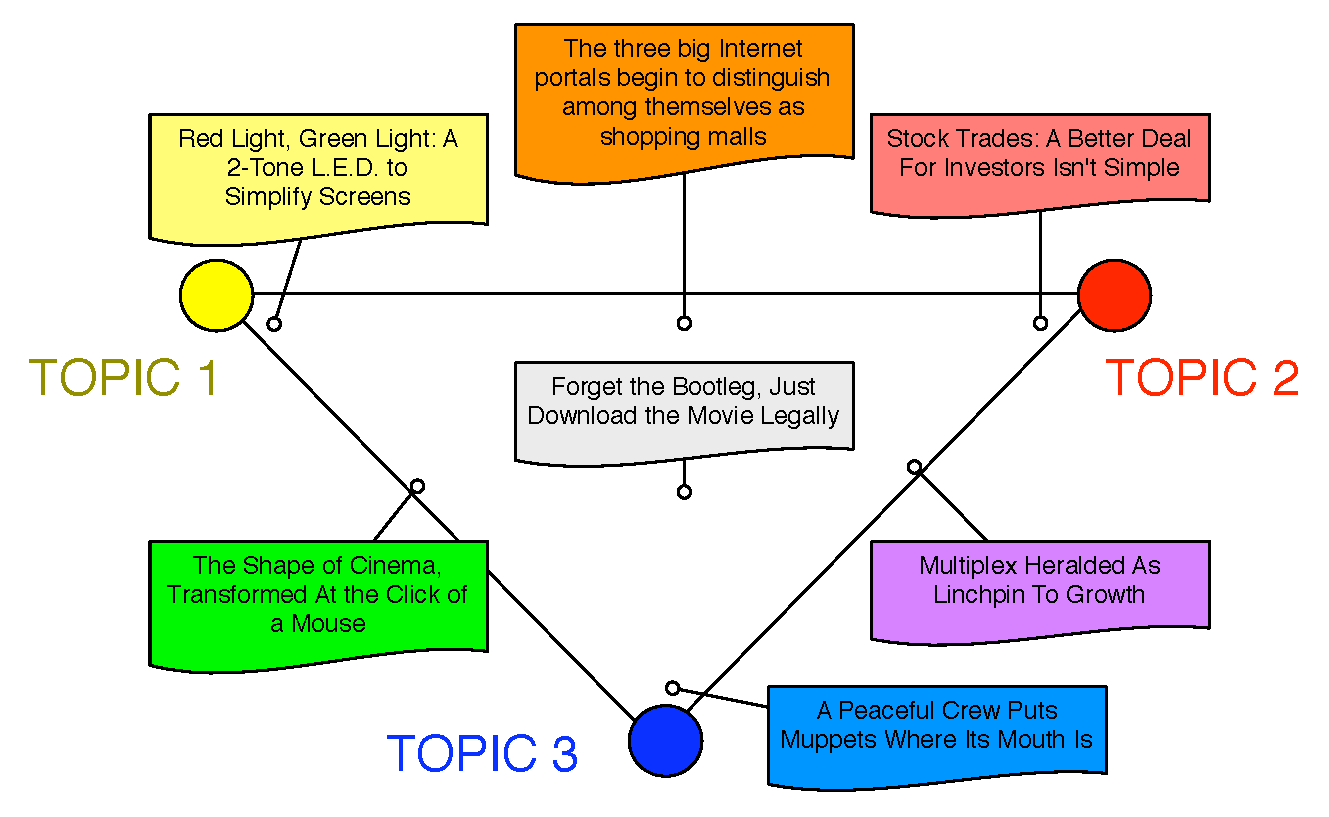
\includegraphics[width=0.9\linewidth]{topic_models/nyt_documents}}
\end{center}

\end{frame}


\begin{frame}{Evaluating Topic Models}

\begin{columns}

\column{.6\linewidth}
\begin{block}{ Reading Tea Leaves: How Humans Interpret Topic Models}
Jonathan Chang, Jordan Boyd-Graber, Chong Wang, Sean Gerrish, and David
M. Blei. Reading Tea Leaves: How Humans Interpret Topic Models. Neural
Information Processing Systems, 2009.
\end{block}

\column{.3\linewidth}
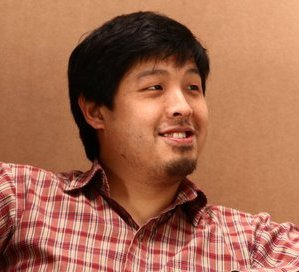
\includegraphics[width=.8\linewidth]{general_figures/jonathan}

\end{columns}

\end{frame}



\frame{
\frametitle{Evaluation}
\begin{center}
%\only<1>{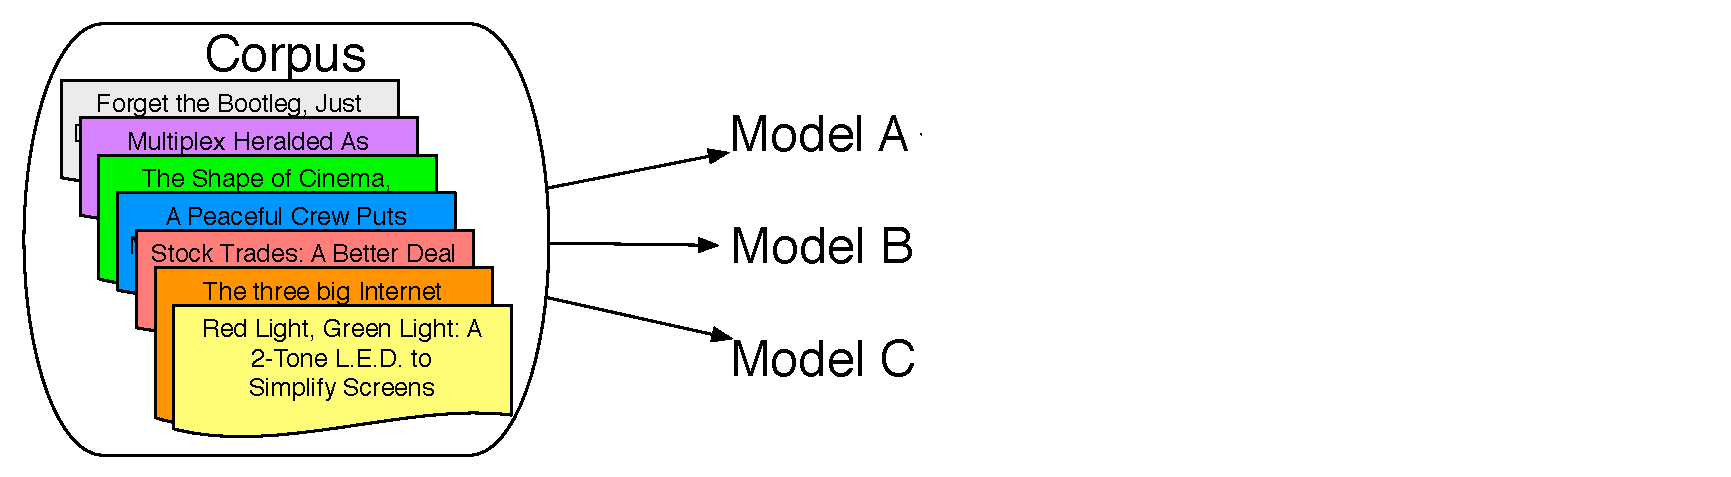
\includegraphics[width=0.9\linewidth]{reading_tea_leaves/figures/heldout_1} }
\only<1>{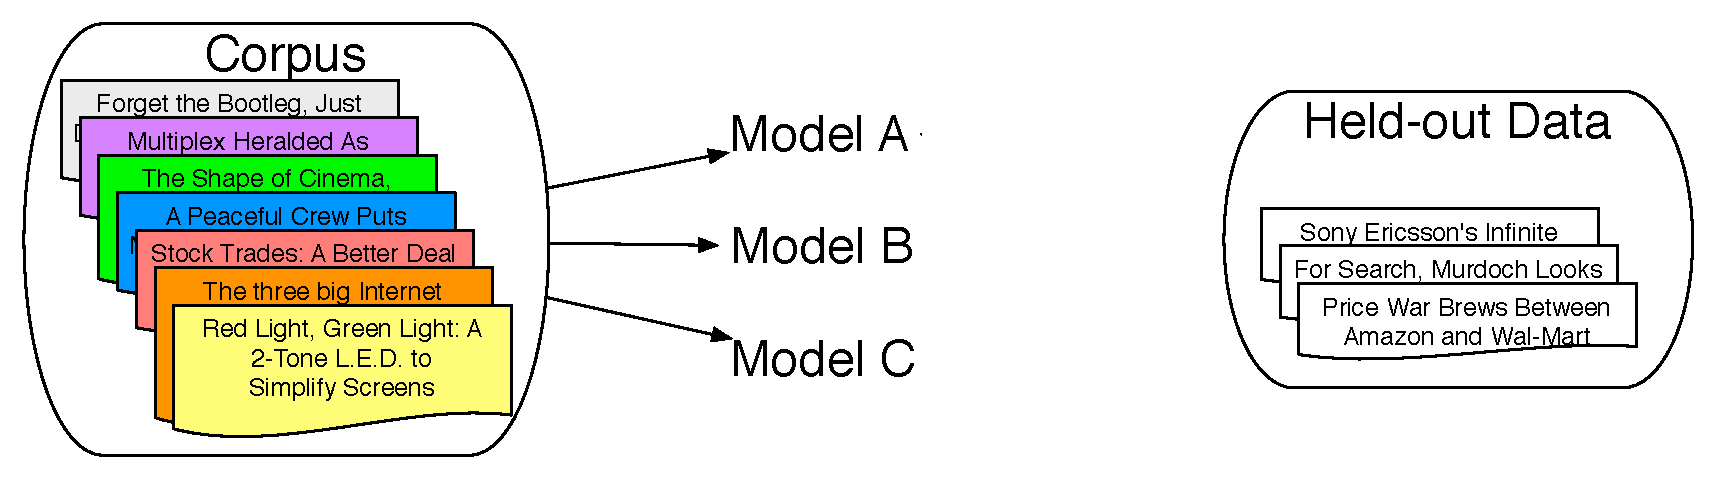
\includegraphics[width=\linewidth]{reading_tea_leaves/figures/heldout_2} }
%\only<3>{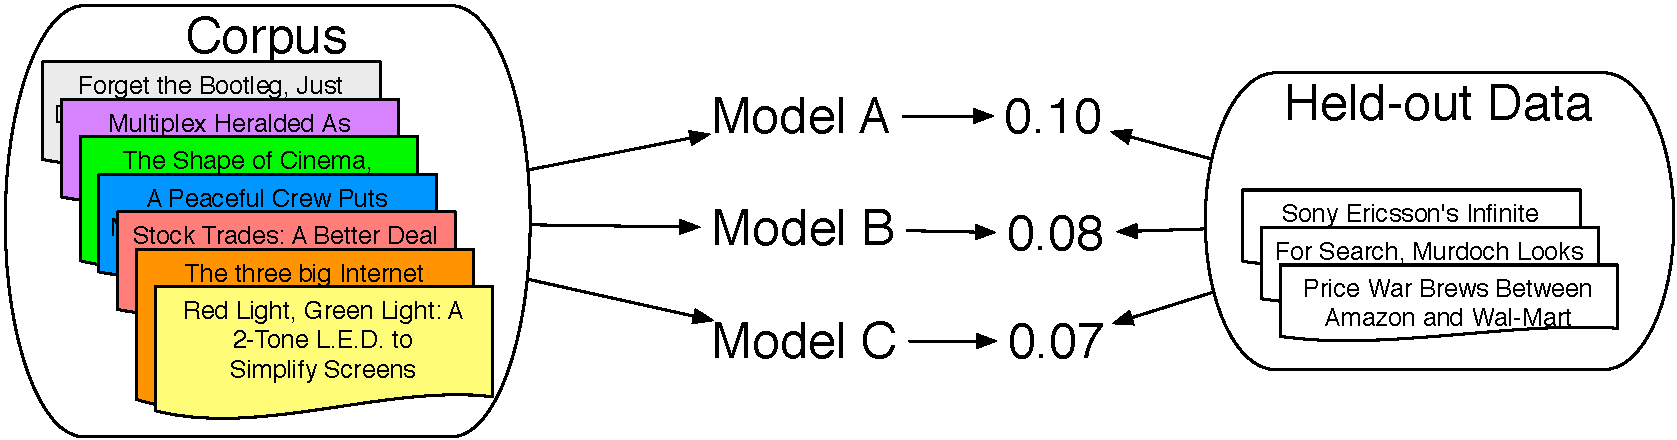
\includegraphics[width=\linewidth]{reading_tea_leaves/figures/heldout_3} }
\only<2>{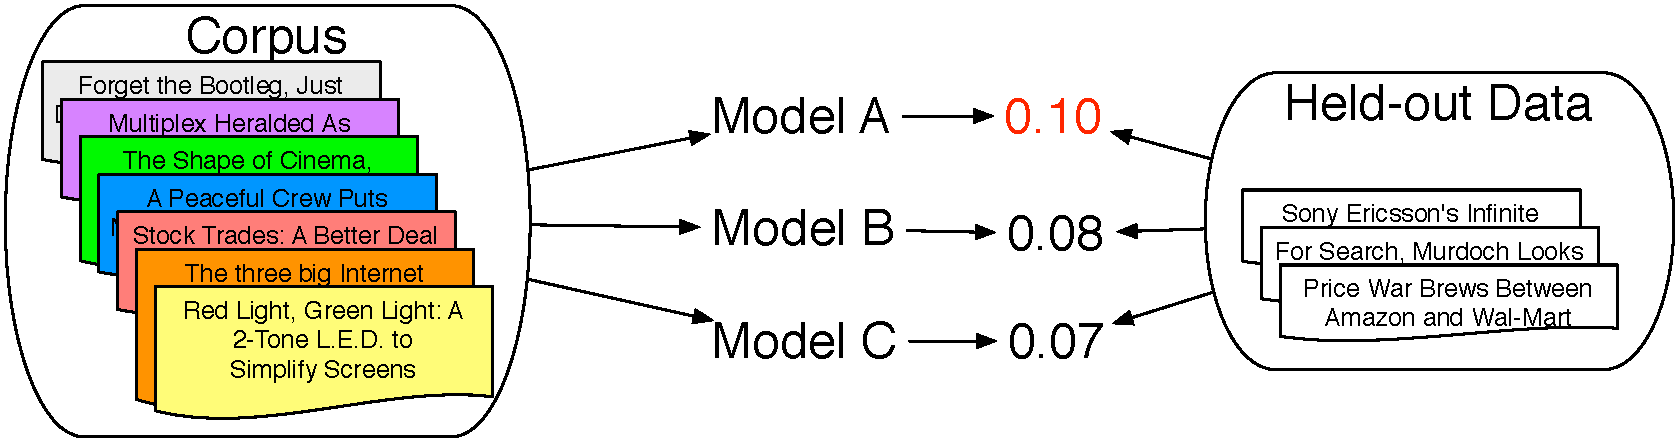
\includegraphics[width=\linewidth]{reading_tea_leaves/figures/heldout_4}  \\
	\large Measures predictive power (likelihood)}
\end{center}
}

\begin{frame}{But we don't use topic models for prediction!}

\gfxs{autocomplete}{.8}

\end{frame}

\frame{
\frametitle{Qualitative Evaluation of the Latent Space}

\begin{center}
\only<1>{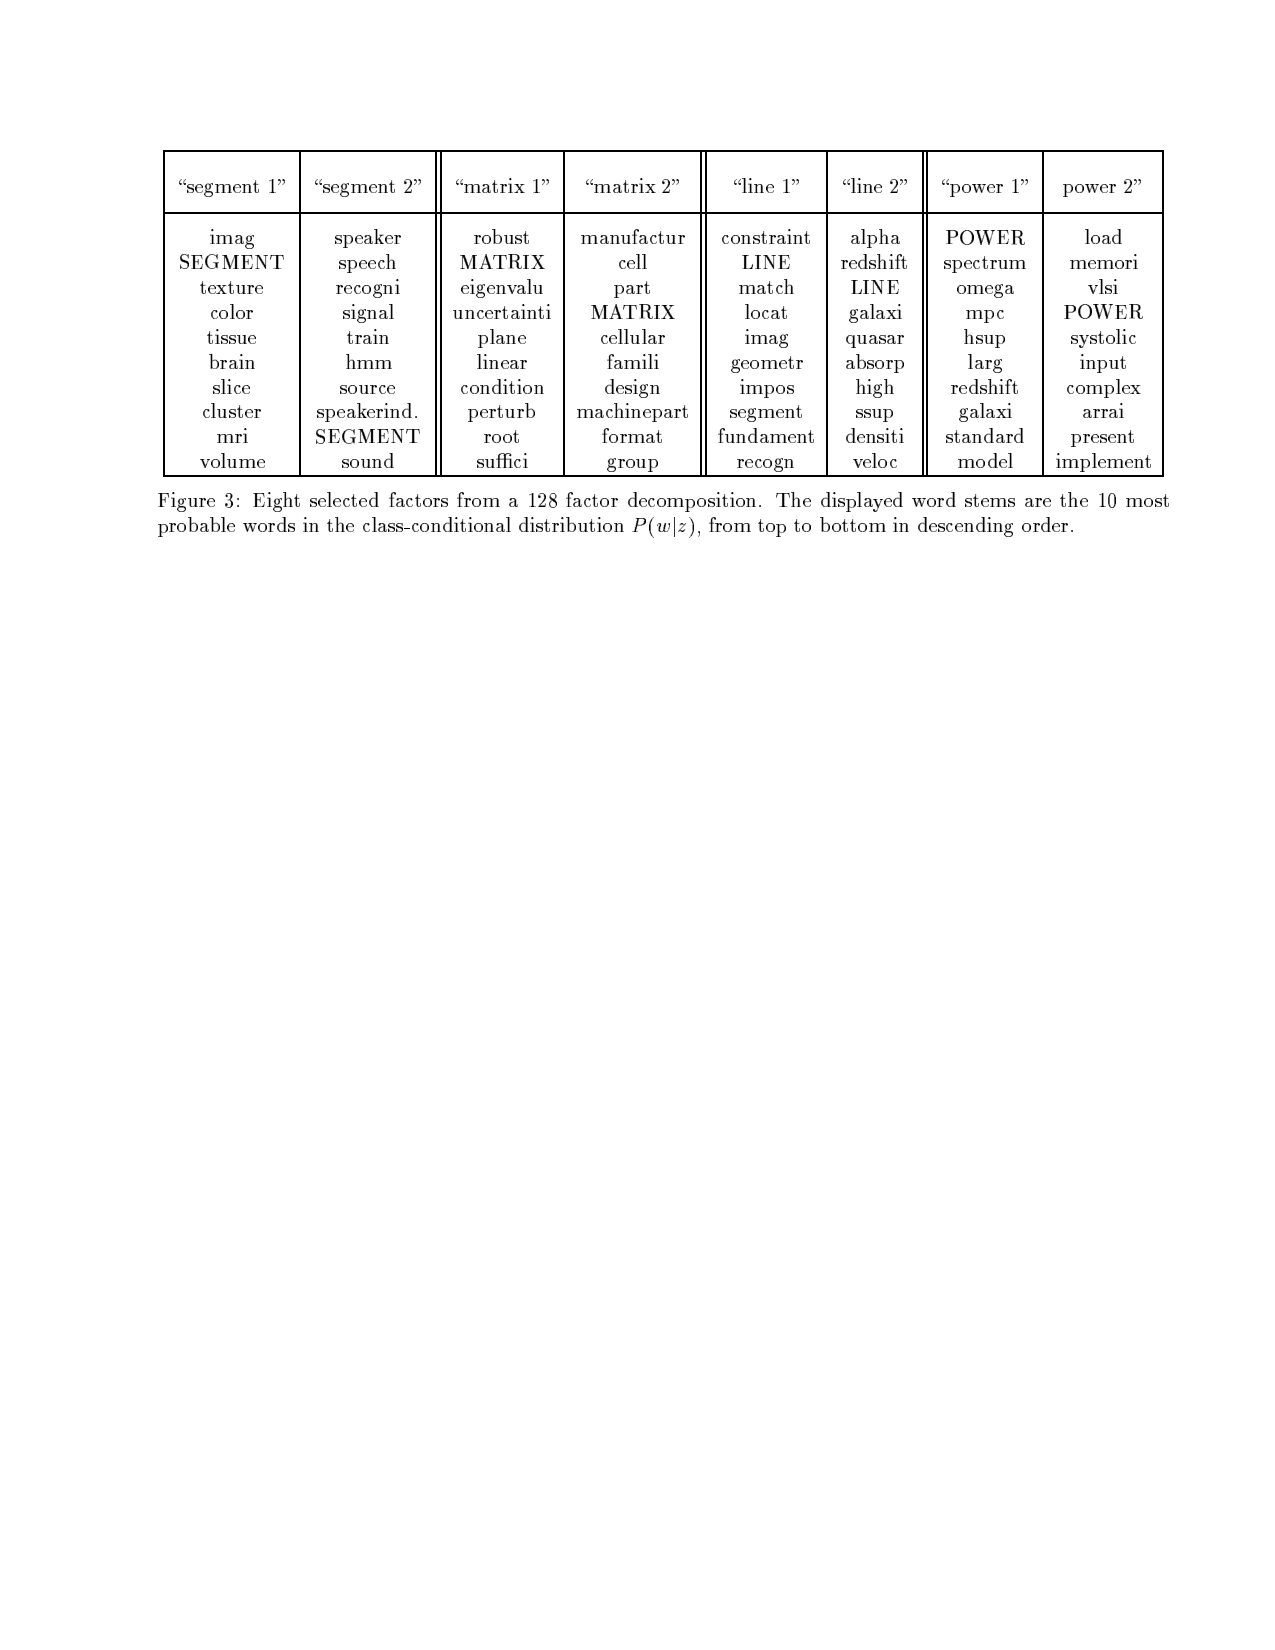
\includegraphics[width=0.9\linewidth]{reading_tea_leaves/topics_from_papers/1} \\ \cite{hofmann-99} }
\only<2>{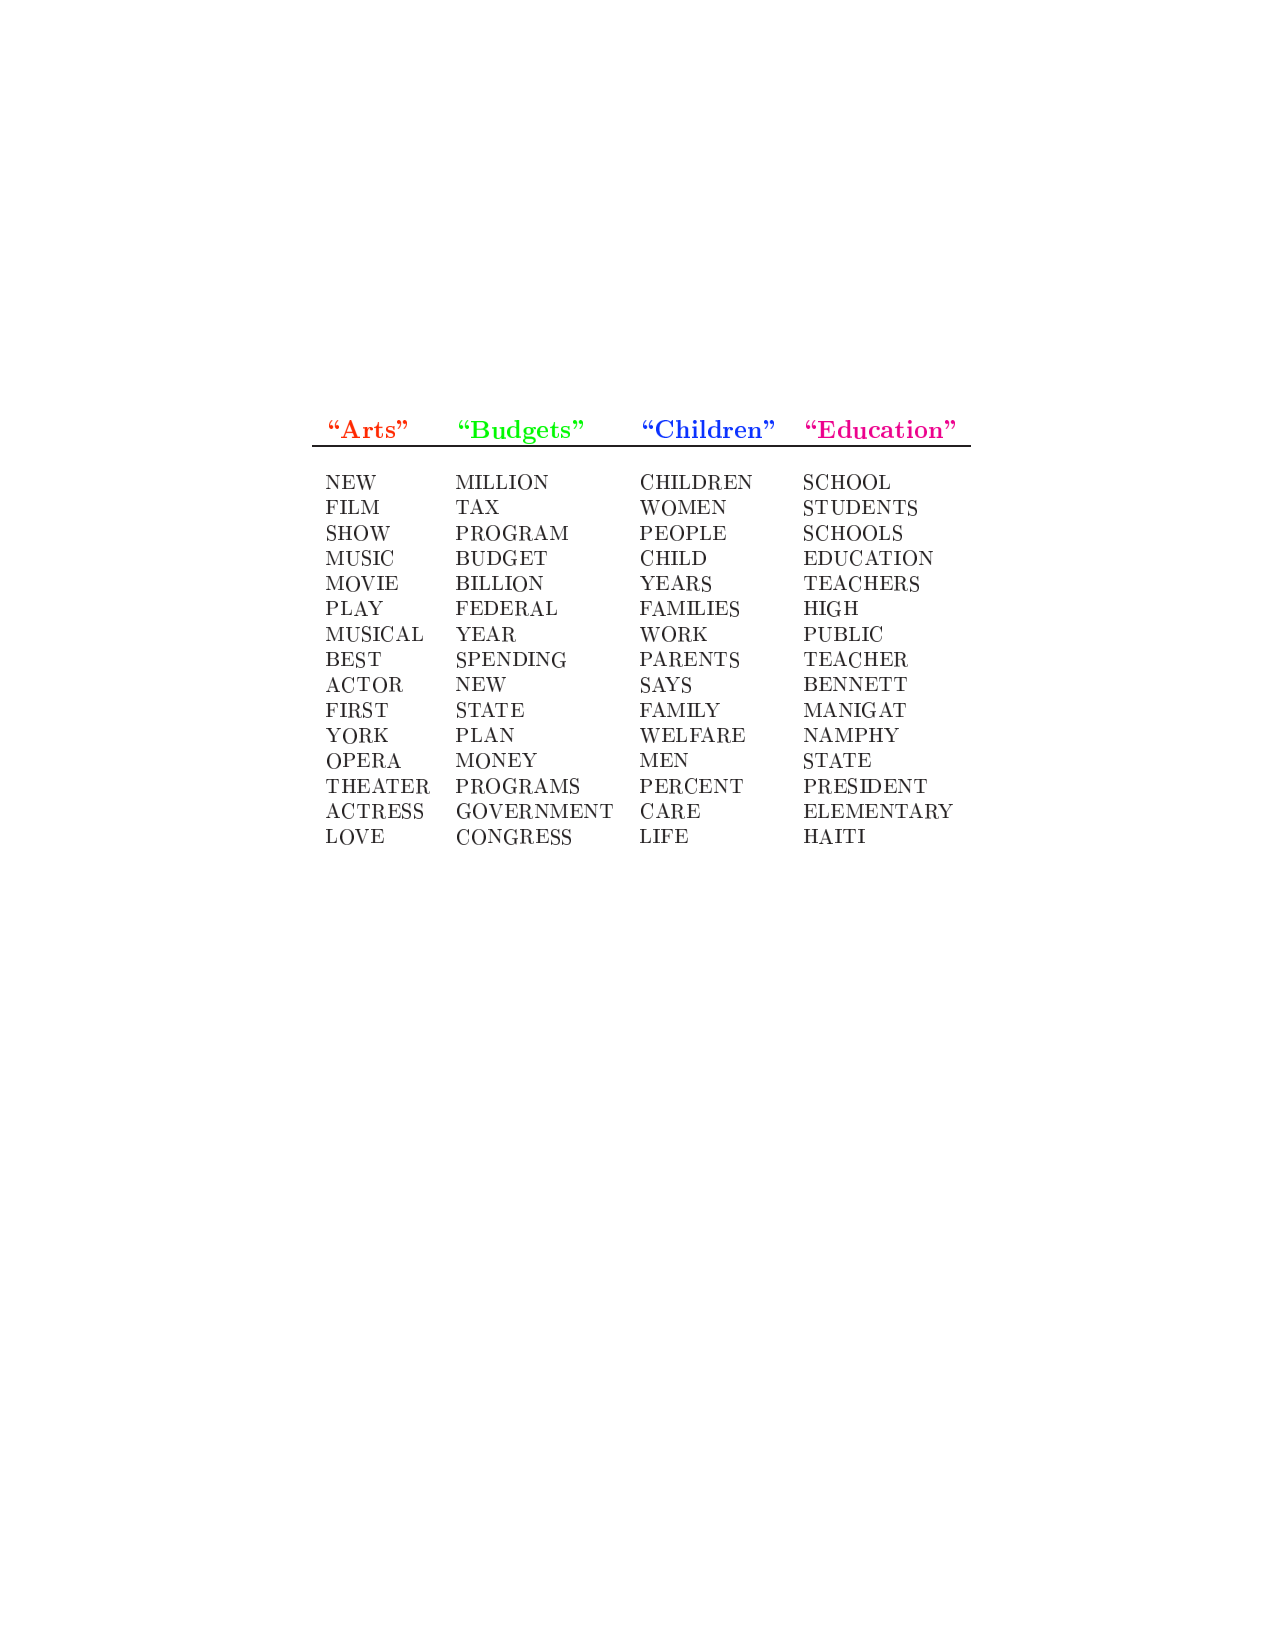
\includegraphics[width=0.7\linewidth]{reading_tea_leaves/topics_from_papers/2} \\ \cite{blei-03} }
\only<3>{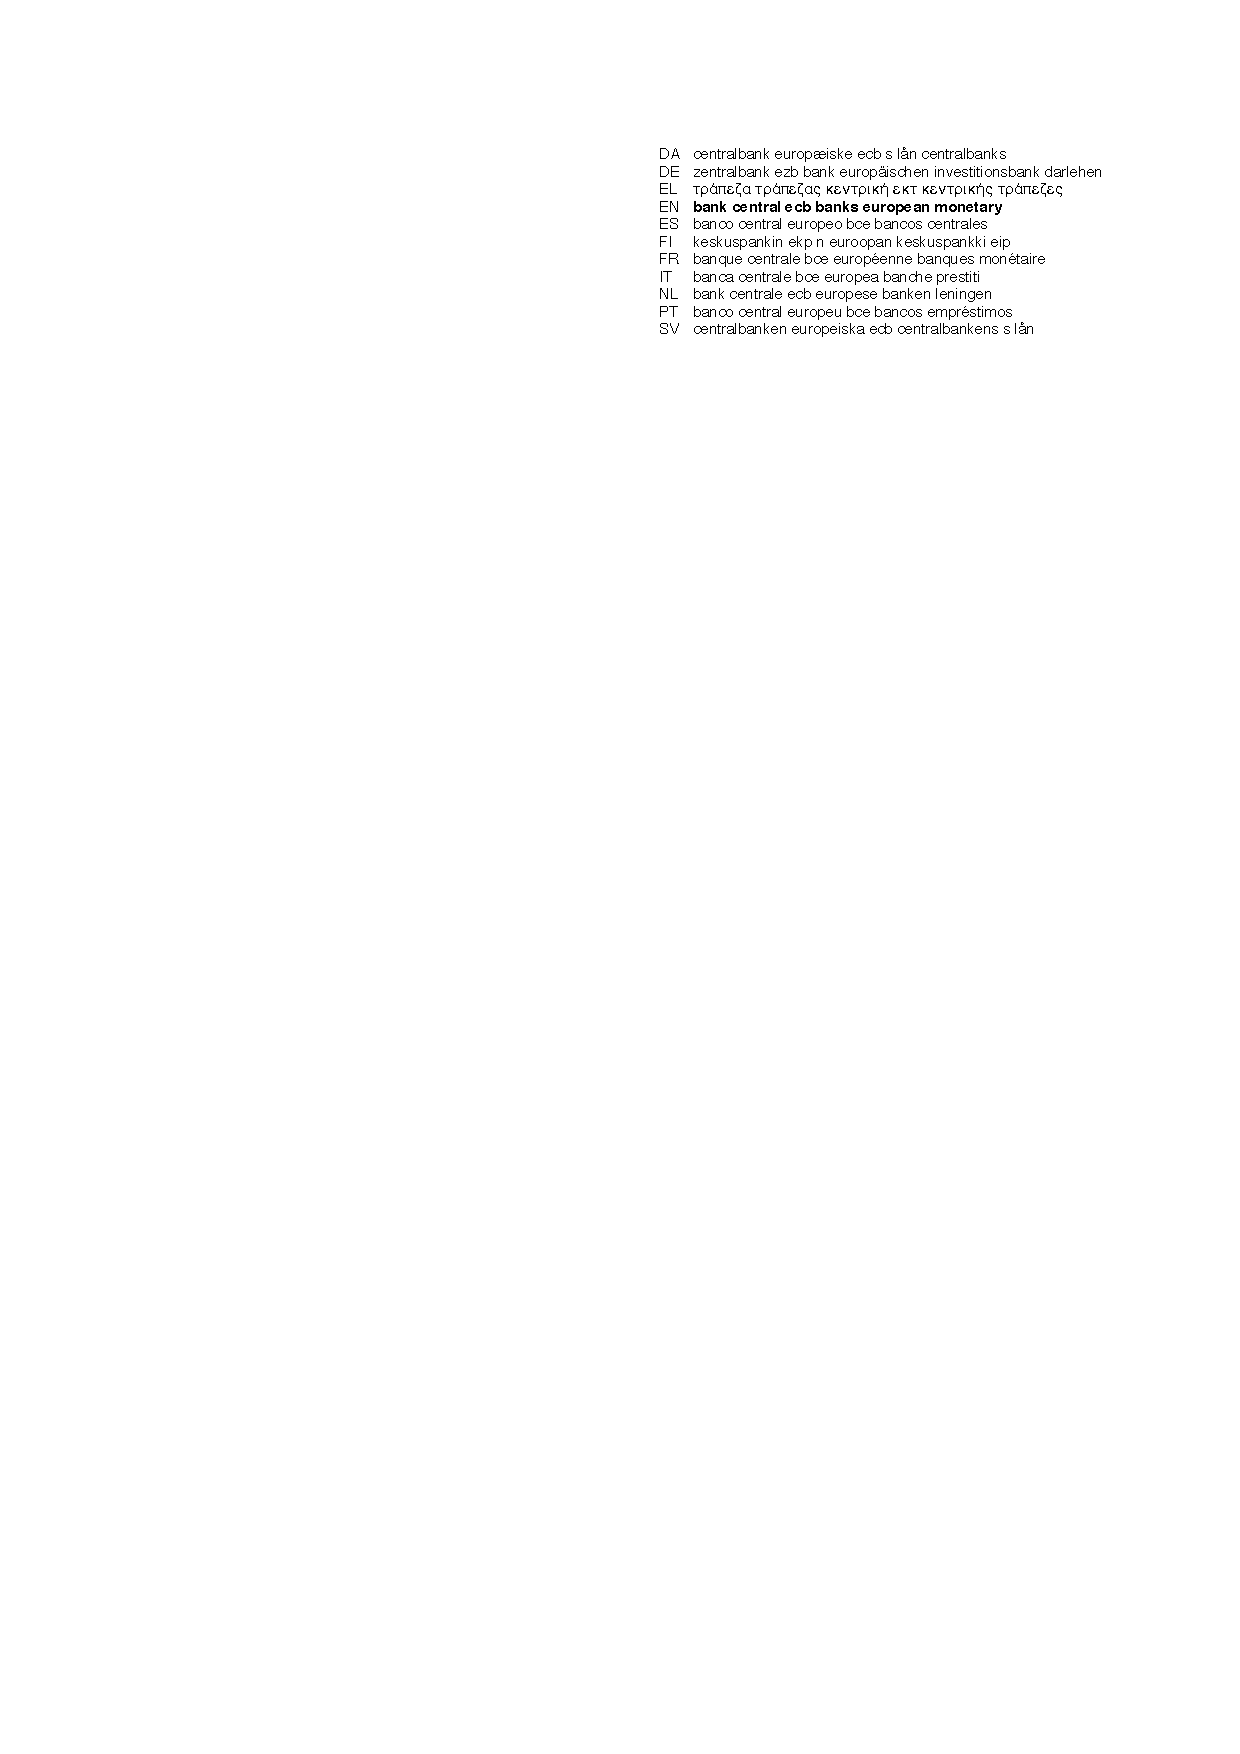
\includegraphics[width=0.7\linewidth]{reading_tea_leaves/topics_from_papers/3} \\ \cite{mimno-09} }
\only<4>{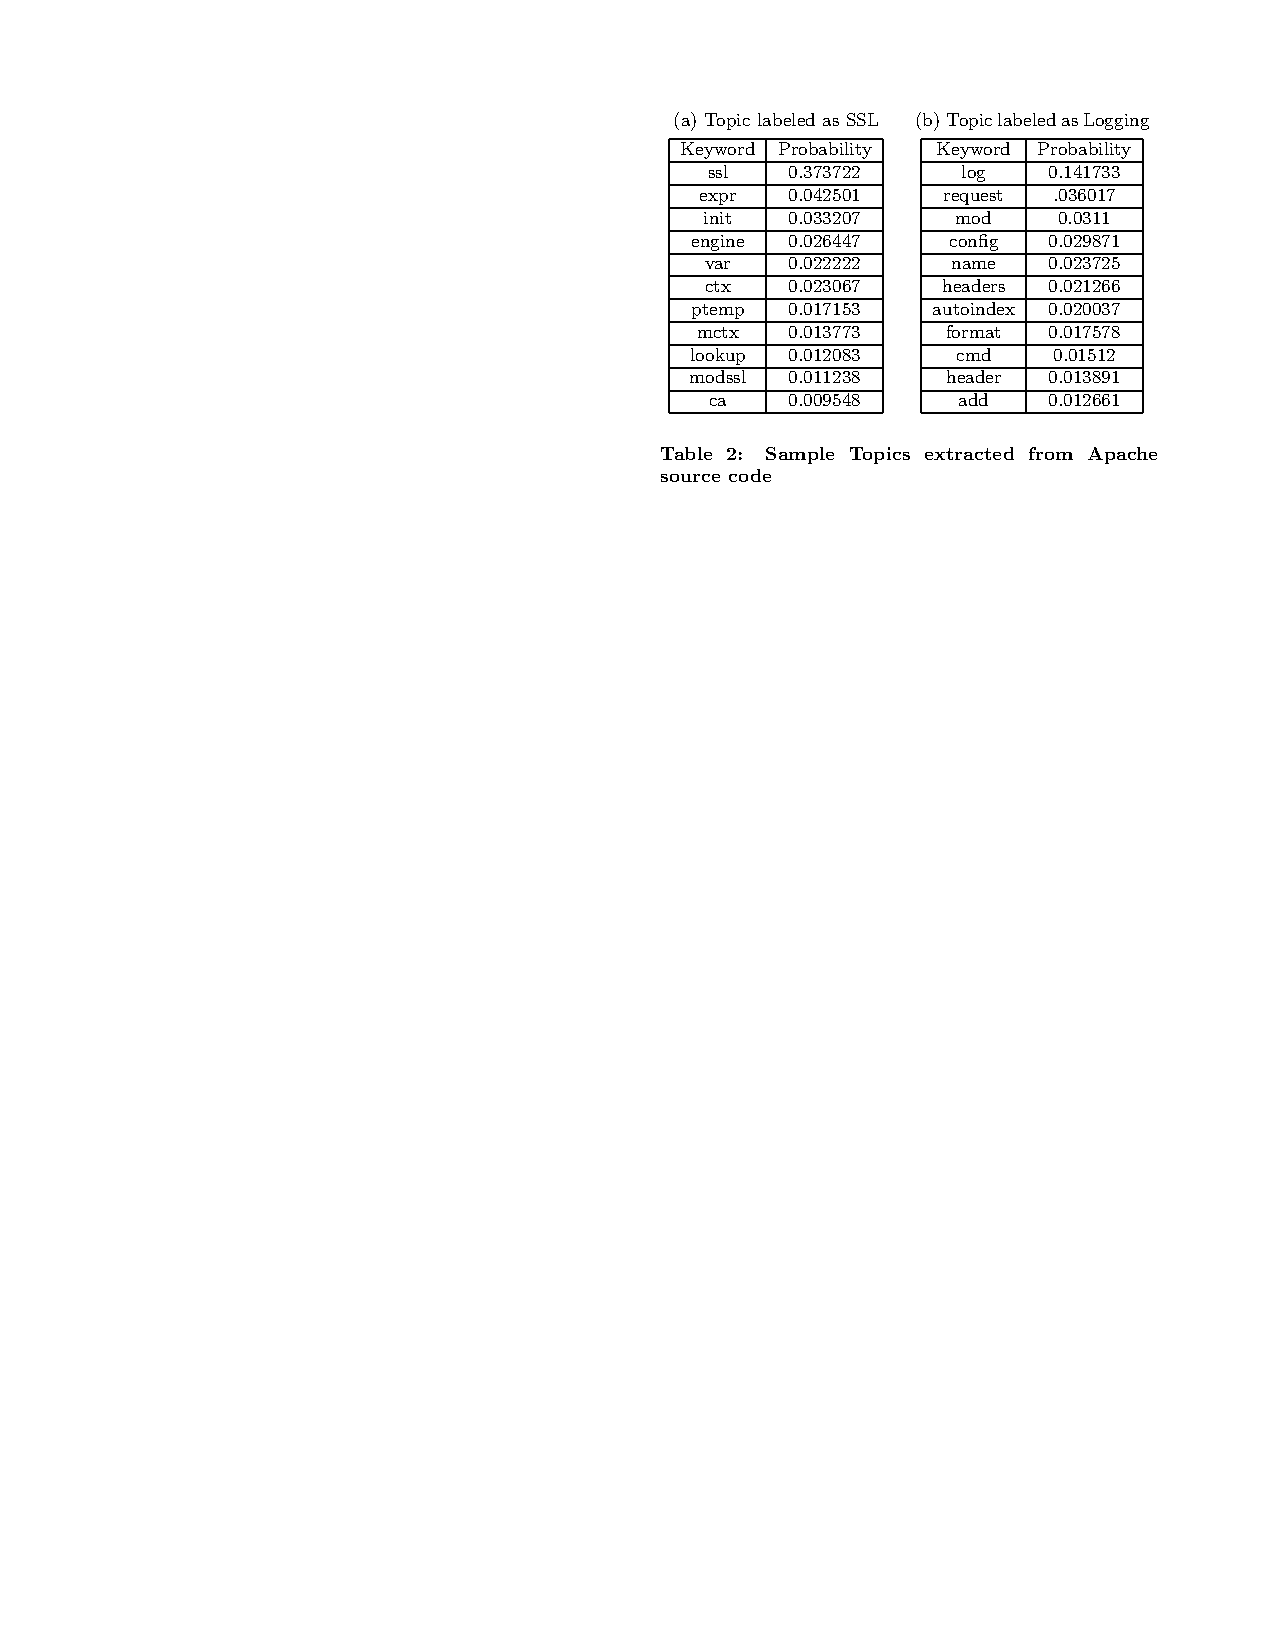
\includegraphics[width=0.7\linewidth]{reading_tea_leaves/topics_from_papers/4}
  \\ \cite{maskeri-08} }
\end{center}
}

\frame{
  \frametitle{Word Intrusion}

  \begin{itemize}
    \item Take the highest probability words from a topic

      \begin{block}{Original Topic}
        dog \\ cat \\ \only<2->{\alert<2->{apple} \\ } horse \\ pig \\ cow
      \end{block}

\only<2->{    \item \alert<2>{Intruder: high probability word from another topic}}
\pause
  \end{itemize}
}

\frame{
\frametitle{Interpretability and Likelihood}


\begin{center}
\only<1>{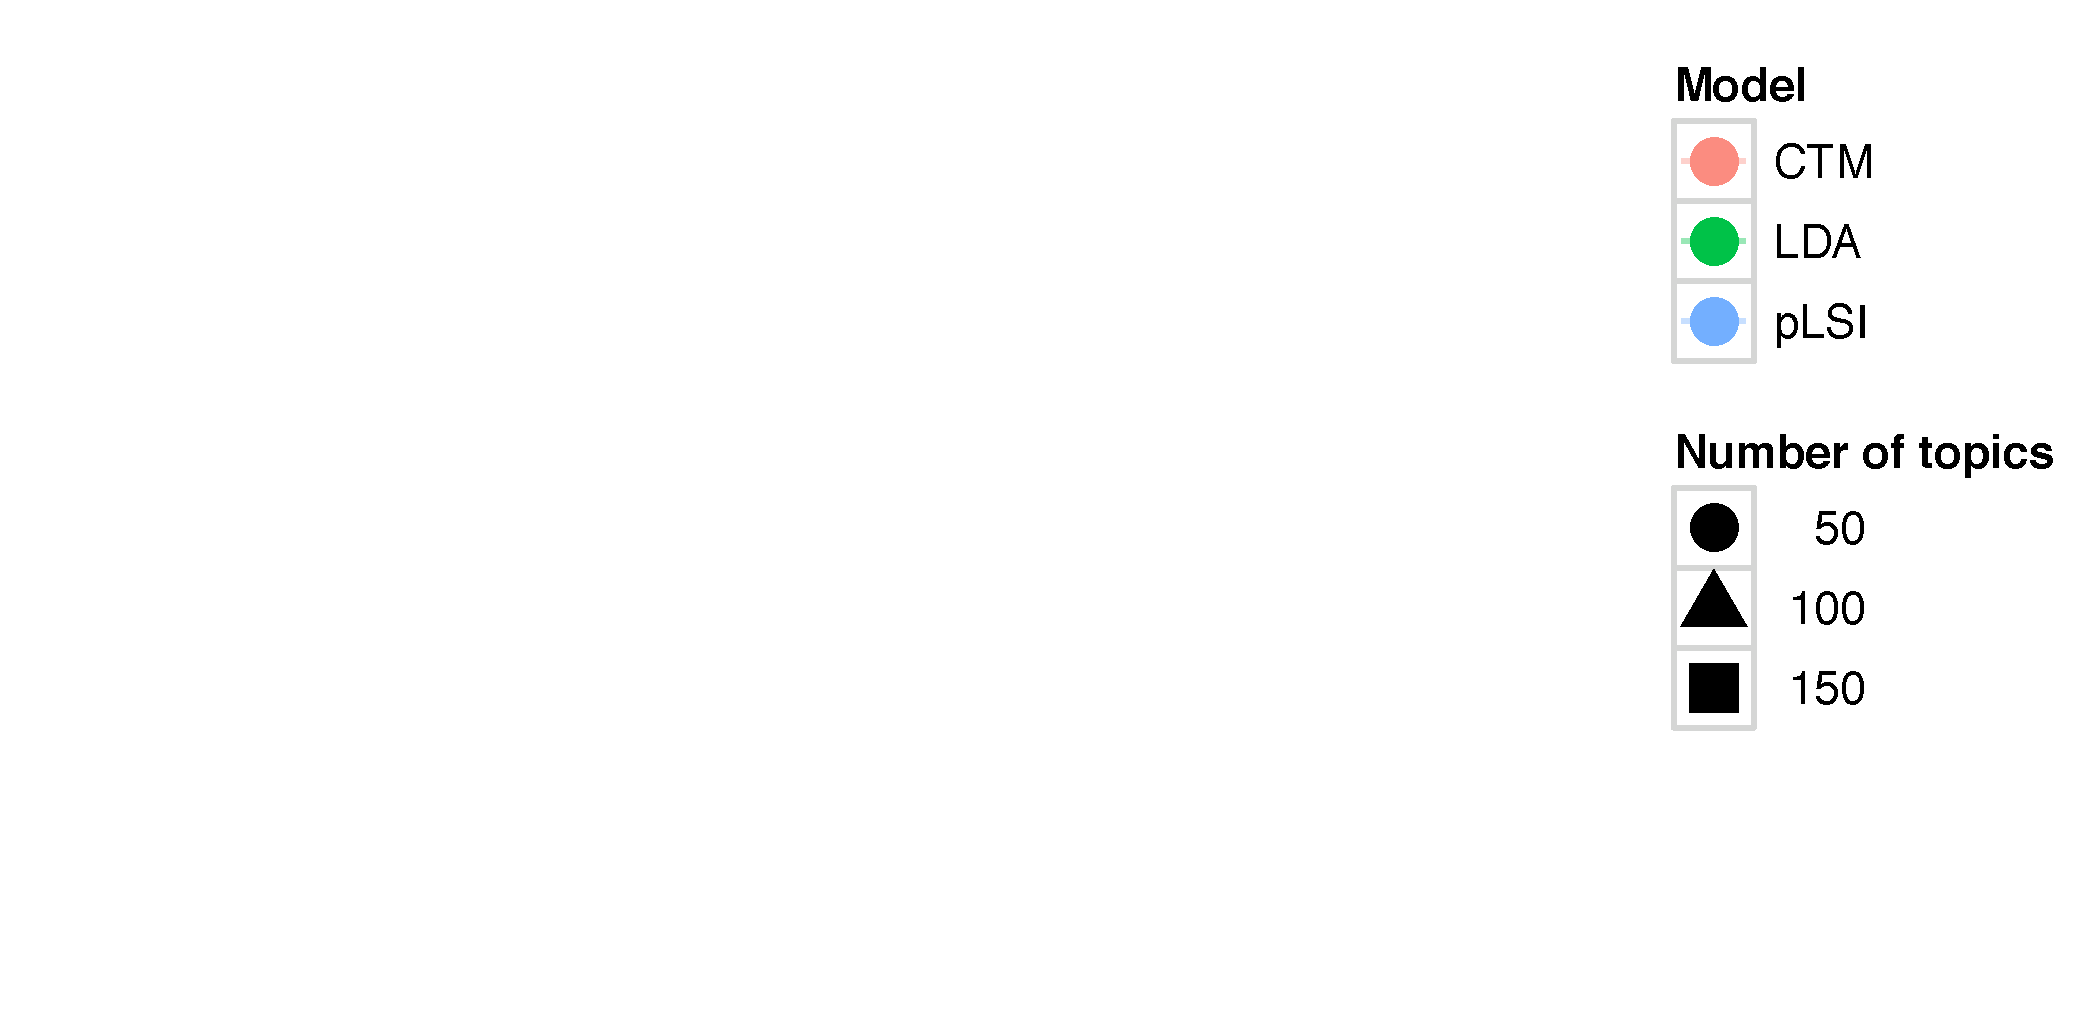
\includegraphics[width=.8\paperwidth]{reading_tea_leaves/figures/prec_ll_1}}
\only<2>{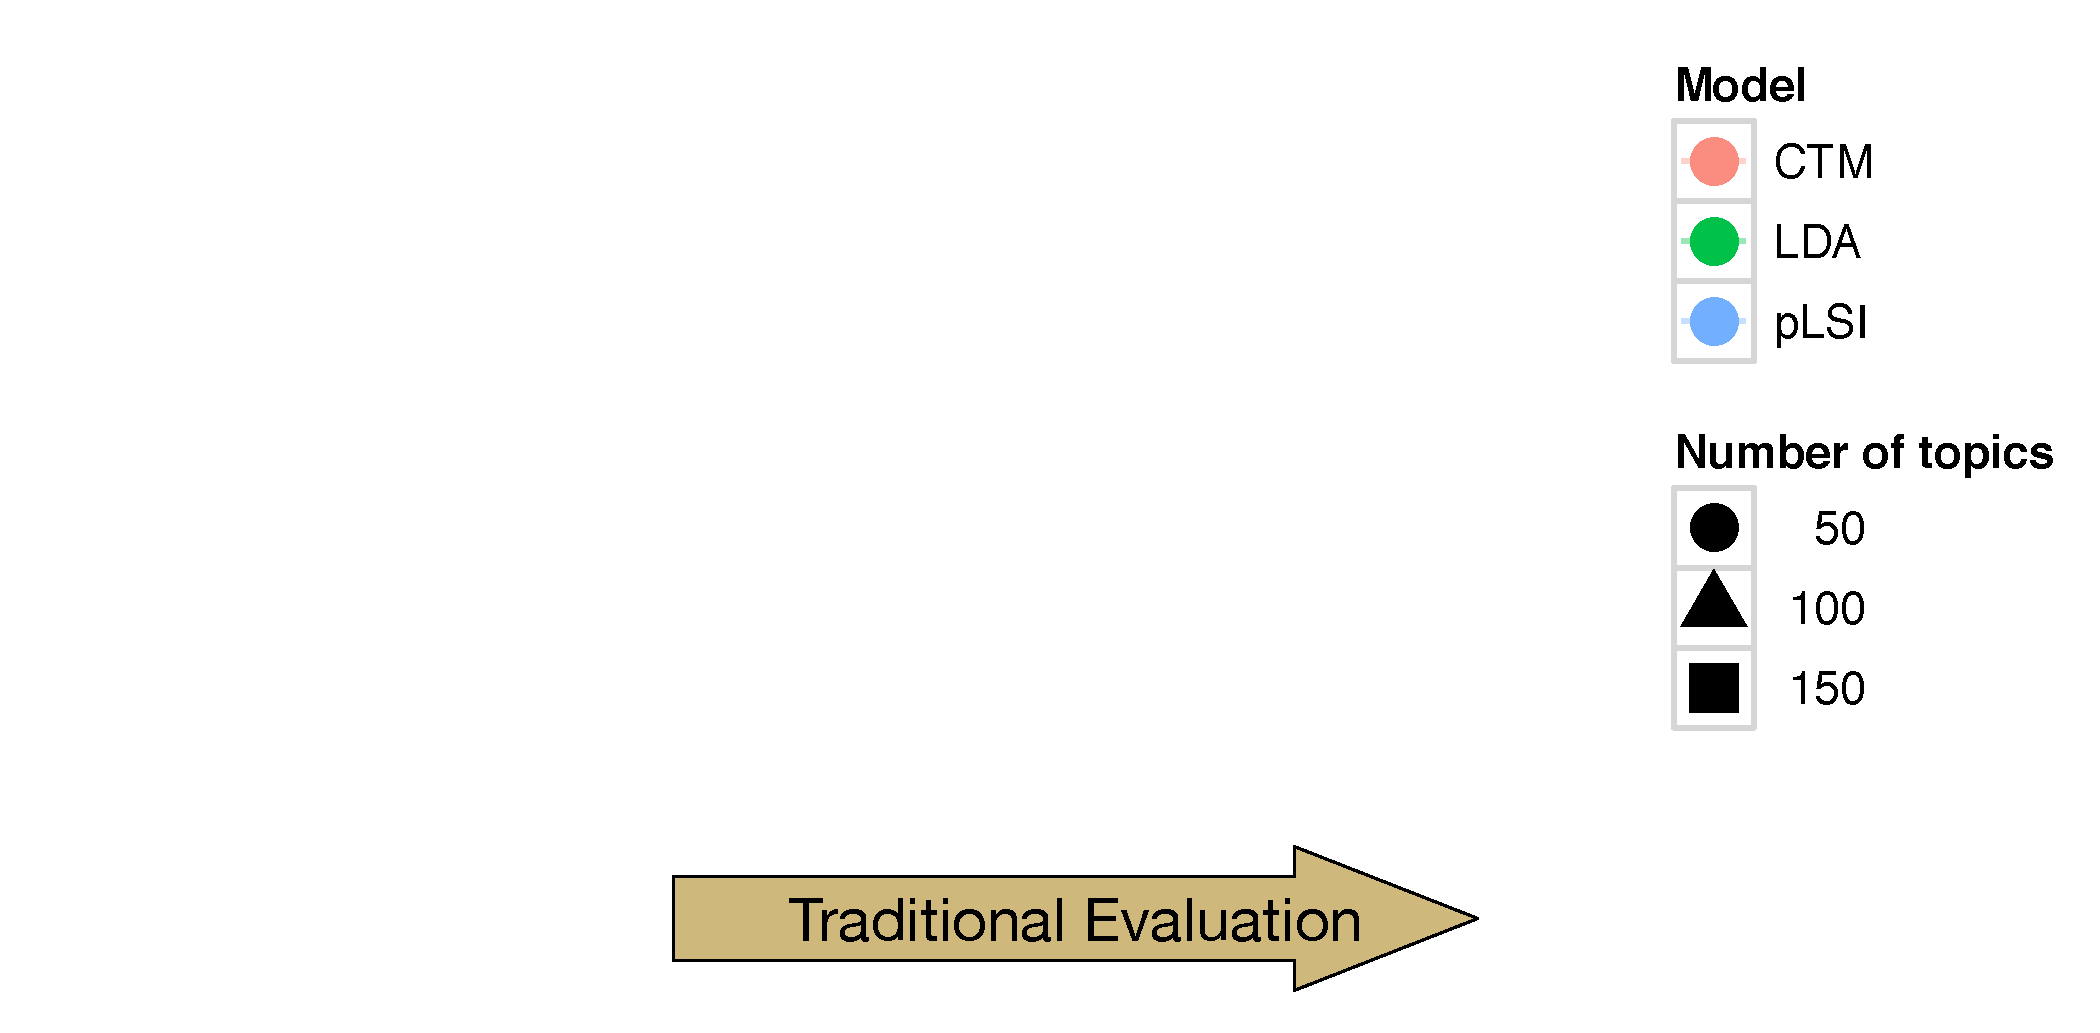
\includegraphics[width=.8\paperwidth]{reading_tea_leaves/figures/prec_ll_2}}
\only<3>{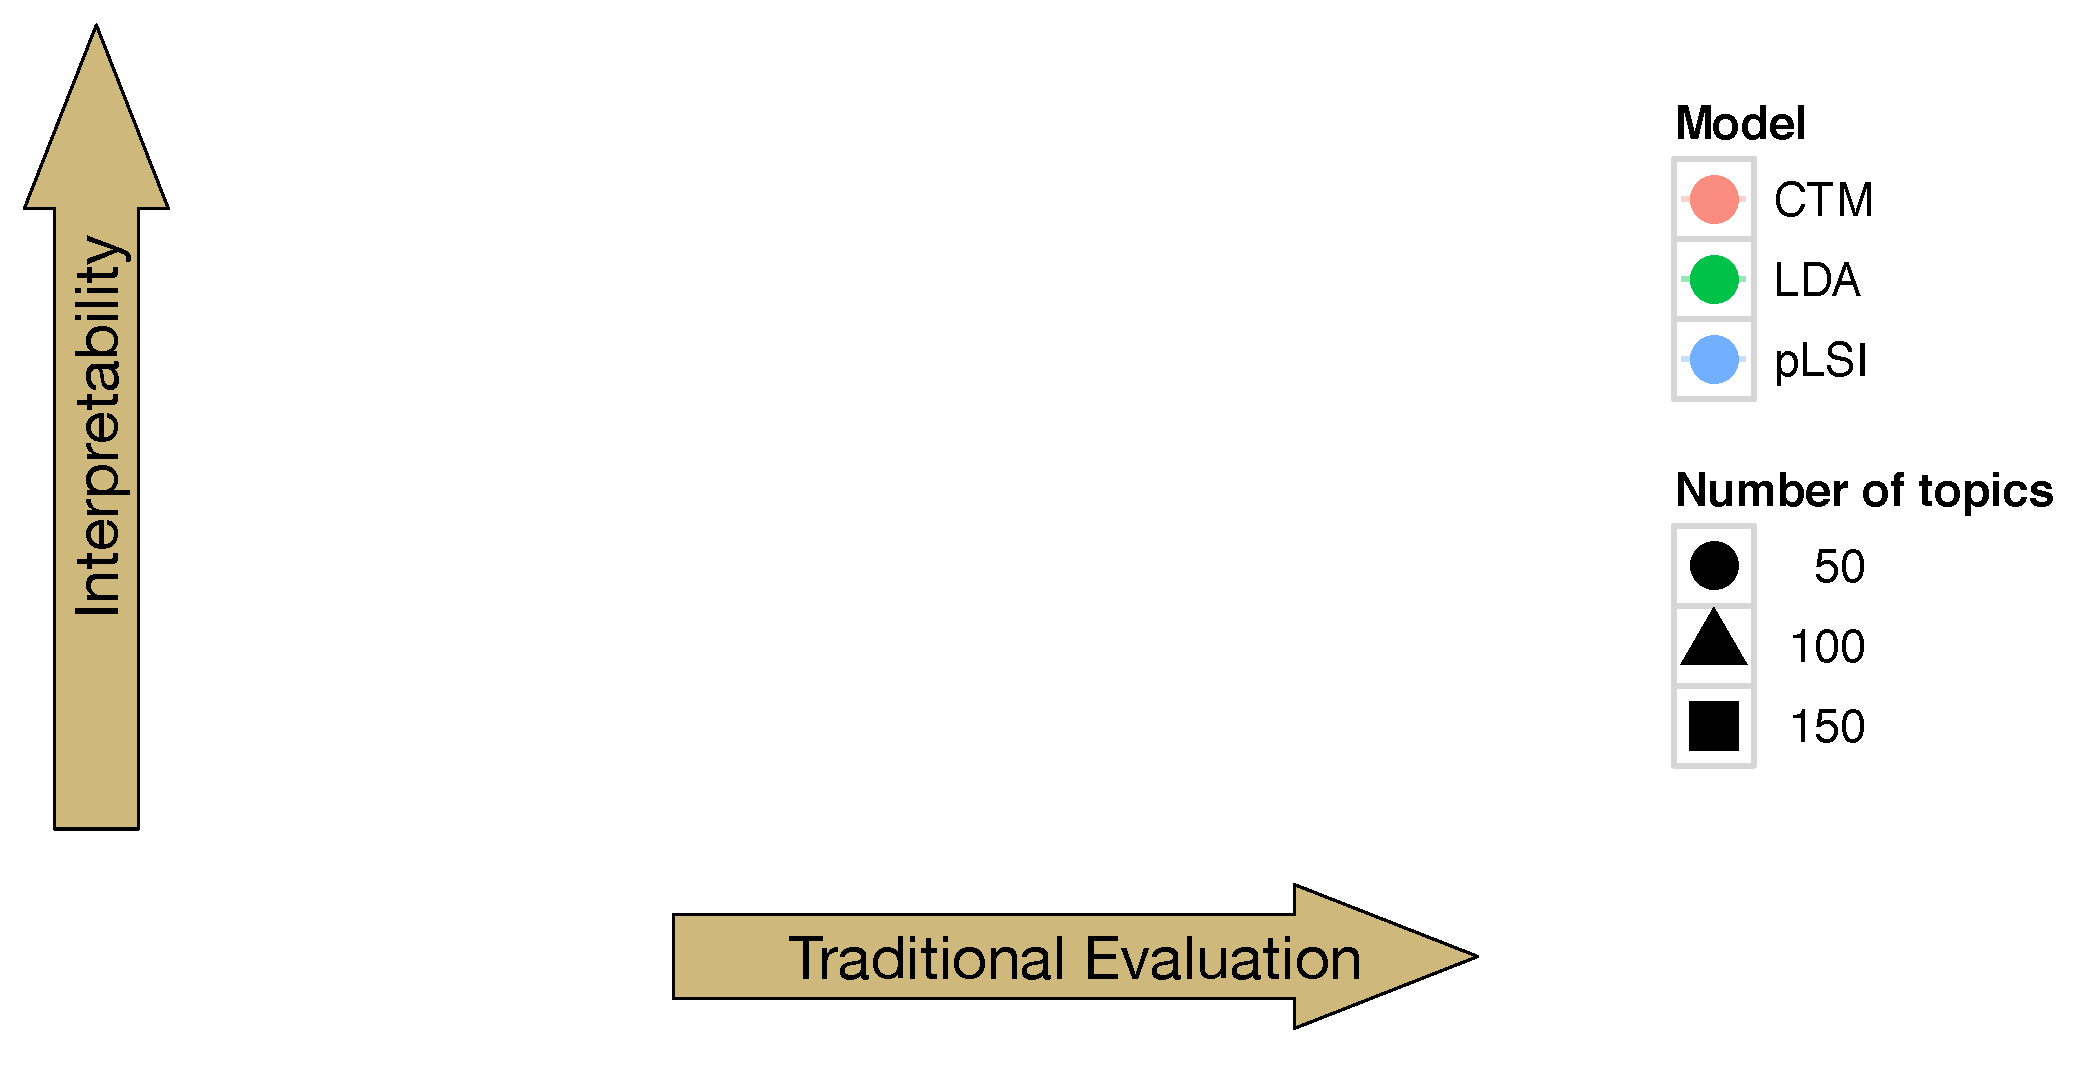
\includegraphics[width=.8\paperwidth]{reading_tea_leaves/figures/prec_ll_3}}
\only<4>{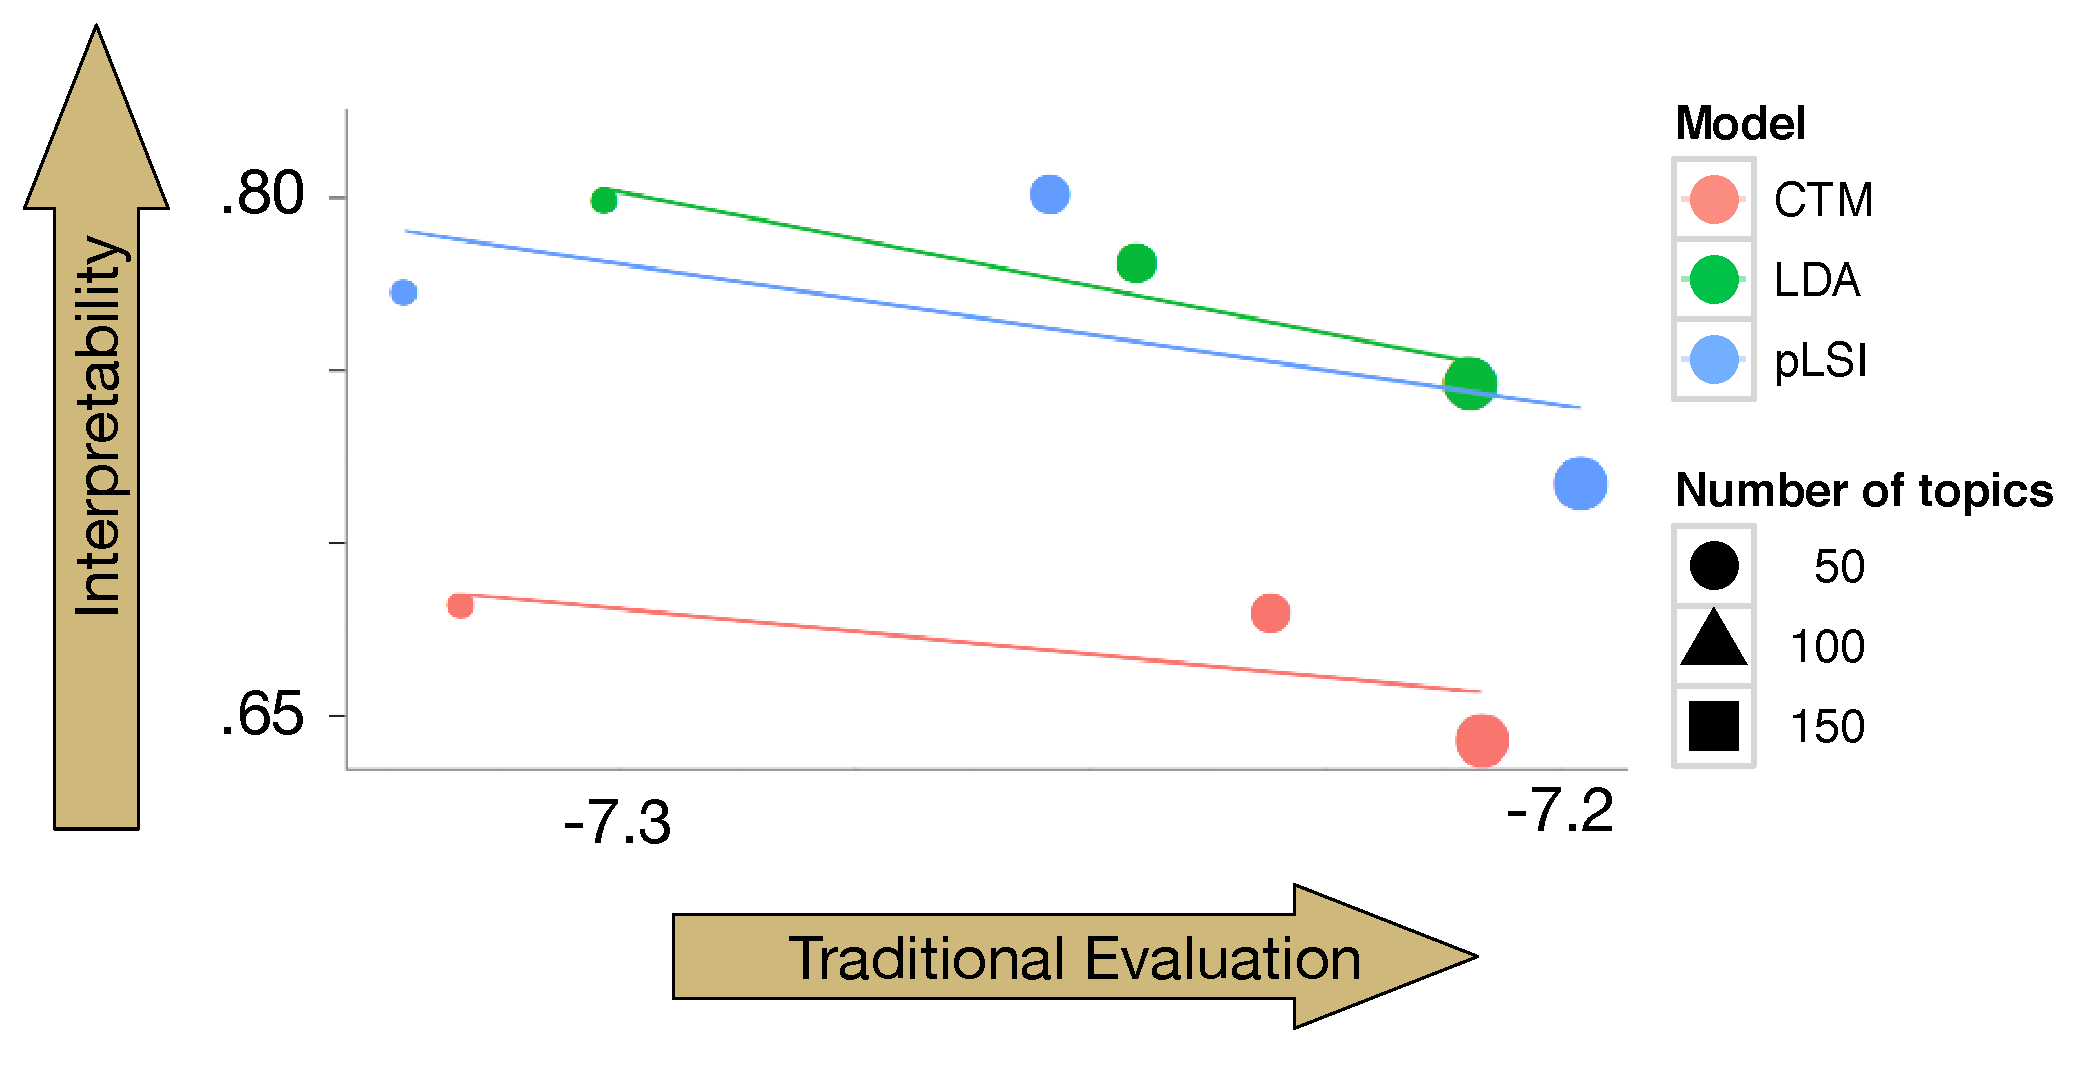
\includegraphics[width=.8\paperwidth]{reading_tea_leaves/figures/prec_ll_4}}
\only<4>{\\ Within a model, higher likelihood $\not =$ higher interpretability}
\end{center}
}


\begin{frame}{Since then \dots}

  \begin{itemize}
    \item A way to get at an evaluation that matches {\bf what we care about}
    \item A necessary step to improving topic models for navigating large datasets~\cite{talley-11}
    \item Others have discovered automatic methods that uncover the same properties~\cite{newman-10,mimno-11}
    \item And extended the technique to structured topics and
      phrases~\cite{lindsey-12,weninger-12}
      \item Iteractive refinement with tree-structured
        priors~\cite{hu-14} and spectral algorithms~\cite{Lund-17}
    \item \alert<2>{Extending to multiple users}~\cite{Felt-15}
      \ifjobtalk (CoNLL Best Paper) \fi
  \end{itemize}

\end{frame}




\begin{frame}{}

  \begin{columns}
    \column{.4\linewidth}
    \begin{center}
        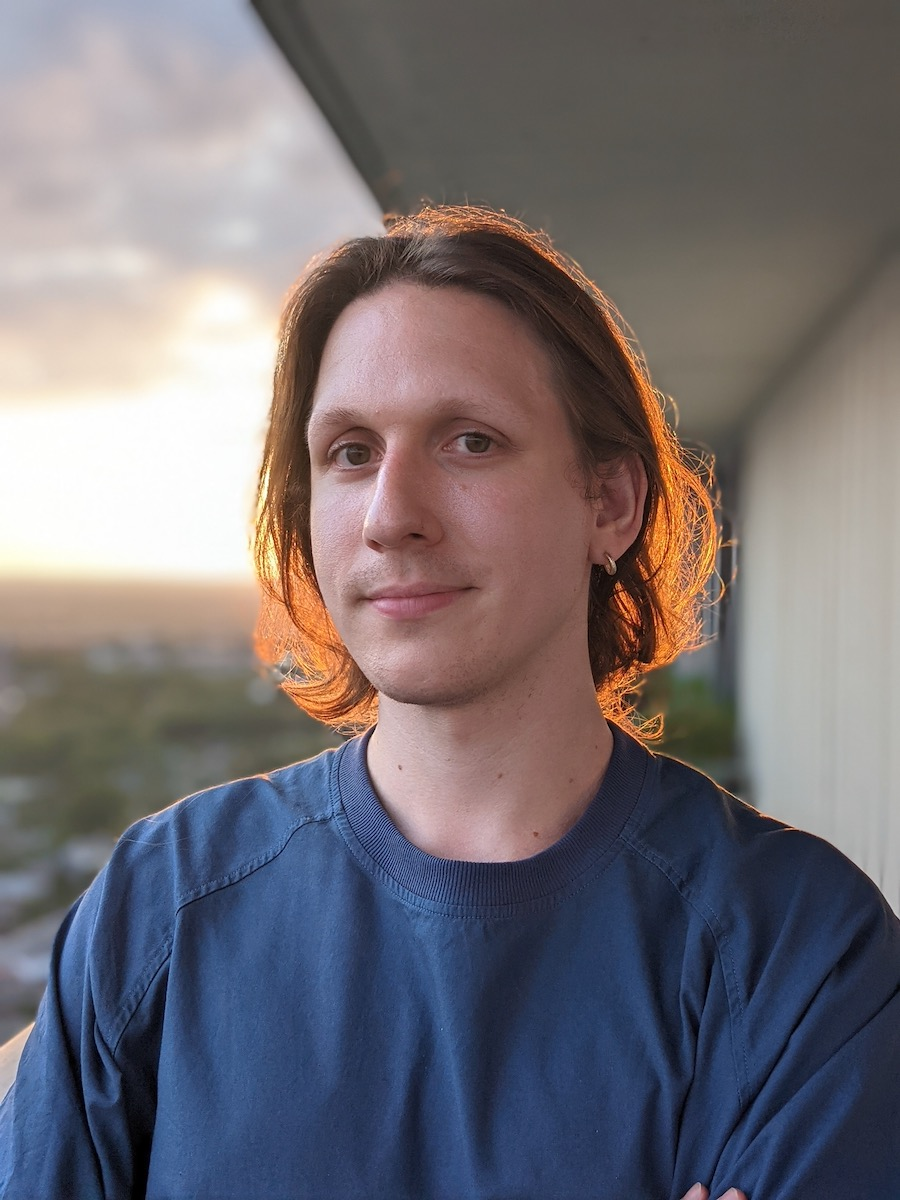
\includegraphics[width=0.8\linewidth]{general_figures/alexander}
        \end{center}
    \column{.6\linewidth}
    \begin{block}{\href{http://umiacs.umd.edu/~jbg//docs/2021_neurips_incoherence.pdf}{Is Automated Topic Evaluation Broken? The Incoherence of Coherence}}
      \href{https://alexanderhoyle.com/}{Alexander Miserlis Hoyle},
      Pranav Goel, Andrew Hian-Cheong, Denis Peskov, Jordan
      Boyd-Graber, and Philip Resnik.
      \emph{Neural Information Processing Systems}, 2021
        \end{block}

  \end{columns}
\end{frame}

\begin{frame}{Is Automatic Coherence Good Enough?}

  \begin{table}
	\centering
		\resizebox{\textheight}{!}{
			\begin{tabular}{lllllllllll}
				\toprule
				Source & Human        & Perplexity & Coherence       & Implementation & Ref. Corpus   & Consistent & Hparam   & >1 run /     & LDA             & Baseline \\
				& Evals?       &            &                 & Specified      & Specified ?   & Preproc?    & search? & err. bars?   & Implementation? & w/in 2 yr?\\
				\midrule
~\cite{Bianchi2020PretrainingIA} & \alert<2>{No} & No & \abr{npmi}, Embed-sim & None & Internal, External-GoogleNews & Yes & No & Yes & Variational & No\\
~\cite{zhao2021neural} & \alert<2>{No} & No & \abr{npmi} & Palmetto & No & Unclear & No & Yes & N/A & Yes\\
~\cite{Feng2020ContextRN} & \alert<2>{No} & Yes & \abr{npmi} & None & No & Yes & No & No & N/A & Yes\\
~\cite{hoyle-etal-2020-improving} & \alert<2>{No} & No & \abr{npmi} & In paper & External \abr{nyt}, Internal & No & Yes & Yes & N/A & Yes\\
~\cite{Hu2020NeuralTM} & \alert<2>{No} & No & $C_p$, $C_a$, \abr{npmi} & Palmetto & External \abr{wiki} & No & Likely no & No & Sampling & Yes\\
~\cite{Isonuma2020TreeStructuredNT} & \alert<2>{No} & Yes & \abr{npmi} & None & No, likely external & Unclear & No & No & Sampling & No\\
~\cite{Joo2020DirichletVA} & \alert<2>{No} & Yes & \abr{npmi} & None & No, likely internal & No & Likely yes & Yes & N/A & Yes\\
~\cite{Lin2020CopulaGN} & \alert<2>{No} & Yes & \abr{npmi} & None & No, likely internal & Unclear & Yes & Yes & N/A & Yes\\
~\cite{Ning2020NonparametricTM} & \alert<2>{No} & Yes & \abr{npmi} & Lau github & No & Yes & Likely no & Yes & Variational & No\\
~\cite{Panwar2020TANNTMTA} & \alert<2>{No} & No & \abr{npmi} & Lau github & No & Yes & Likely no & No & Sampling & Yes\\
~\cite{Rezaee2020ADV} & \alert<2>{No} & No & N/A & N/A & N/A & Yes & Likely no & Yes & Variational & No\\
~\cite{Thompson2020TopicMW} & \alert<2>{No} & No & Coherence, \abr{pmi} & In paper & External \abr{nyt} & \alert<2>{No} & No & Yes & Sampling & No\\
~\cite{Tian2020LearningVM} & \alert<2>{No} & Yes & \abr{npmi} & None & No & No & Yes & No & Variational & Yes\\
~\cite{Wang2020NeuralTM} & \alert<2>{No} & No & $C_p$, $C_a$, \abr{npmi}, UCI & Palmetto & No & No & No & No & Sampling & Yes\\
~\cite{Wu2020NeuralMC} & \alert<2>{No} & Yes & \abr{npmi} & None & No & No & Yes & No & N/A & Yes\\
~\cite{Wu2020ShortTT} & \alert<2>{No} & No & $C_v$ & Palmetto & No & Yes & No & No & Unspecified & Yes\\
~\cite{Yang2020GraphAT} & \alert<2>{No} & Yes & Coherence & In paper & No, likely internal & Yes & No & No & Unspecified & No\\
~\cite{Zhou2020NeuralTM} & \alert<2>{No} & No & \abr{npmi}, $C_p$ & Palmetto & External \abr{wiki} & No & Likely no & No & Unspecified & Yes\\
~\cite{burkhardtDecouplingSparsitySmoothness2019} & \alert<2>{No} & Yes & \abr{npmi} & None & No, likely internal & Unclear & Yes & No & Variational & Yes\\
~\cite{diengTopicModelingEmbedding2019} & \alert<2>{No} & Yes & Coherence & In paper & No, likely internal & Yes & No & No & Unspecified & No\\
~\cite{Gui2019NeuralTM} & \alert<2>{No} & No & $C_v$ & None & External \abr{wiki} & Yes & Likely no & No & Unspecified & Yes\\
~\cite{Gupta2019DocumentIN} & \alert<2>{No} & Yes & $C_v$ & Gensim & No, likely internal & Unclear & Likely no & No & N/A & No\\
~\cite{Gupta2019textTOvecDC} & \alert<2>{No} & Yes & $C_v$ & Gensim & No, likely internal & Unclear & Likely no & No & Sampling & Yes\\
~\cite{Lin2019SparsemaxAR} & \alert<2>{No} & Yes & PMI & In paper & No, likely external & Unclear & No & No & Variational & Yes\\
~\cite{Liu2019NeuralVC} & \alert<2>{No} & Yes & \abr{npmi} & Lau github & No, likely internal & Yes & No & No & Variational & Yes\\
~\cite{Nan2019TopicMW} & \alert<2>{No} & No & \abr{npmi} & None & No & No & No & No & Sampling & Yes\\
~\cite{Wang2019ATMAT} & \alert<2>{No} & No & $C_p$, $C_a$, UCI, \abr{npmi}, UMASS & Palmetto & No & No & No & No & Unspecified & Yes\\
~\cite{Card2018NeuralMF} & \alert<2>{No} & Yes & \abr{npmi} & In paper & External-gigaword & Yes & Likely yes & No & Sampling & Yes\\
~\cite{Ding2018CoherenceAwareNT} & \alert<2>{No} & Yes & \abr{npmi} & Lau github & No, likely external & No & Likely no & No & Sampling & Yes\\
~\cite{He2018InteractionAwareTM} & \alert<2>{No} & No & Coherence & None & No, likely internal & Yes & No & No & N/A & Yes\\
~\cite{Peng2018NeuralST} & \alert<2>{No} & Yes & N/A & N/A & N/A & Yes & Likely no & No & Variational & Yes\\
~\cite{Silveira2018TopicMU} & \alert<2>{No} & Yes & \abr{npmi} & Lau github & Internal & Yes & No & Yes & N/A & Yes\\
~\cite{Zhang2018WHAIWH} & \alert<2>{No} & Yes & N/A & N/A & N/A & Unclear & Likely no & No & N/A & Yes\\
~\cite{Zhao2018DirichletBN} & \alert<2>{No} & Yes & \abr{npmi} & Palmetto & External \abr{wiki} & Unclear & No & Yes & N/A & Yes\\
~\cite{Zhu2018GraphBTMGE} & \alert<2>{No} & No & Coherence & None & No, likely internal & Yes & Likely no & No & Variational & Yes\\
~\cite{Jung2017ContinuousST} & \alert<2>{No} & Yes & \abr{npmi}, \abr{PMI}, UMASS & None & No & Yes & No & No & Sampling & Yes\\
~\cite{Miao2017DiscoveringDL} & \alert<2>{No} & Yes & \abr{npmi} & In paper & No & No & Likely no & No & Variational & Yes\\
~\cite{Srivastava2017AutoencodingVI} & \alert<2>{No} & Yes & \abr{npmi} & None & No & Yes & No & No & Sampling & Yes\\
~\cite{Miao2016NeuralVI} & \alert<2>{No} & Yes & N/A & N/A & N/A & Yes & Likely no & No & Unspecified & Yes\\
~\cite{Nguyen2015ImprovingTM} & \alert<2>{No} & No & \abr{npmi} & Lau github & External \abr{wiki} & Yes & No & Yes & Sampling & No\\
				\bottomrule
			\end{tabular}
		}
	\caption{Papers used in meta-analysis}
\end{table}

\end{frame}


\fsi{reading_tea_leaves/incoherence/model_comparison_boxplot}{All that
passes automatic evaluations is not Gold}


\begin{frame}{What about Supervised Models?}

\begin{center}
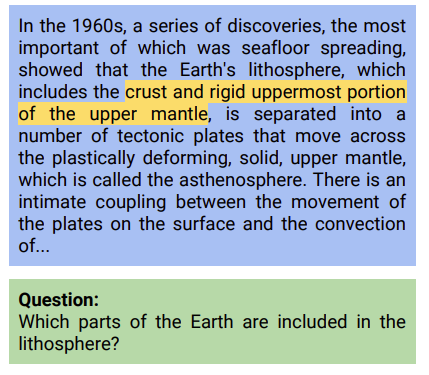
\includegraphics[width=.6\paperwidth]{qb/squad_ex}
\end{center}

\end{frame}


\begin{frame}[plain]
  \vspace{-2cm}
		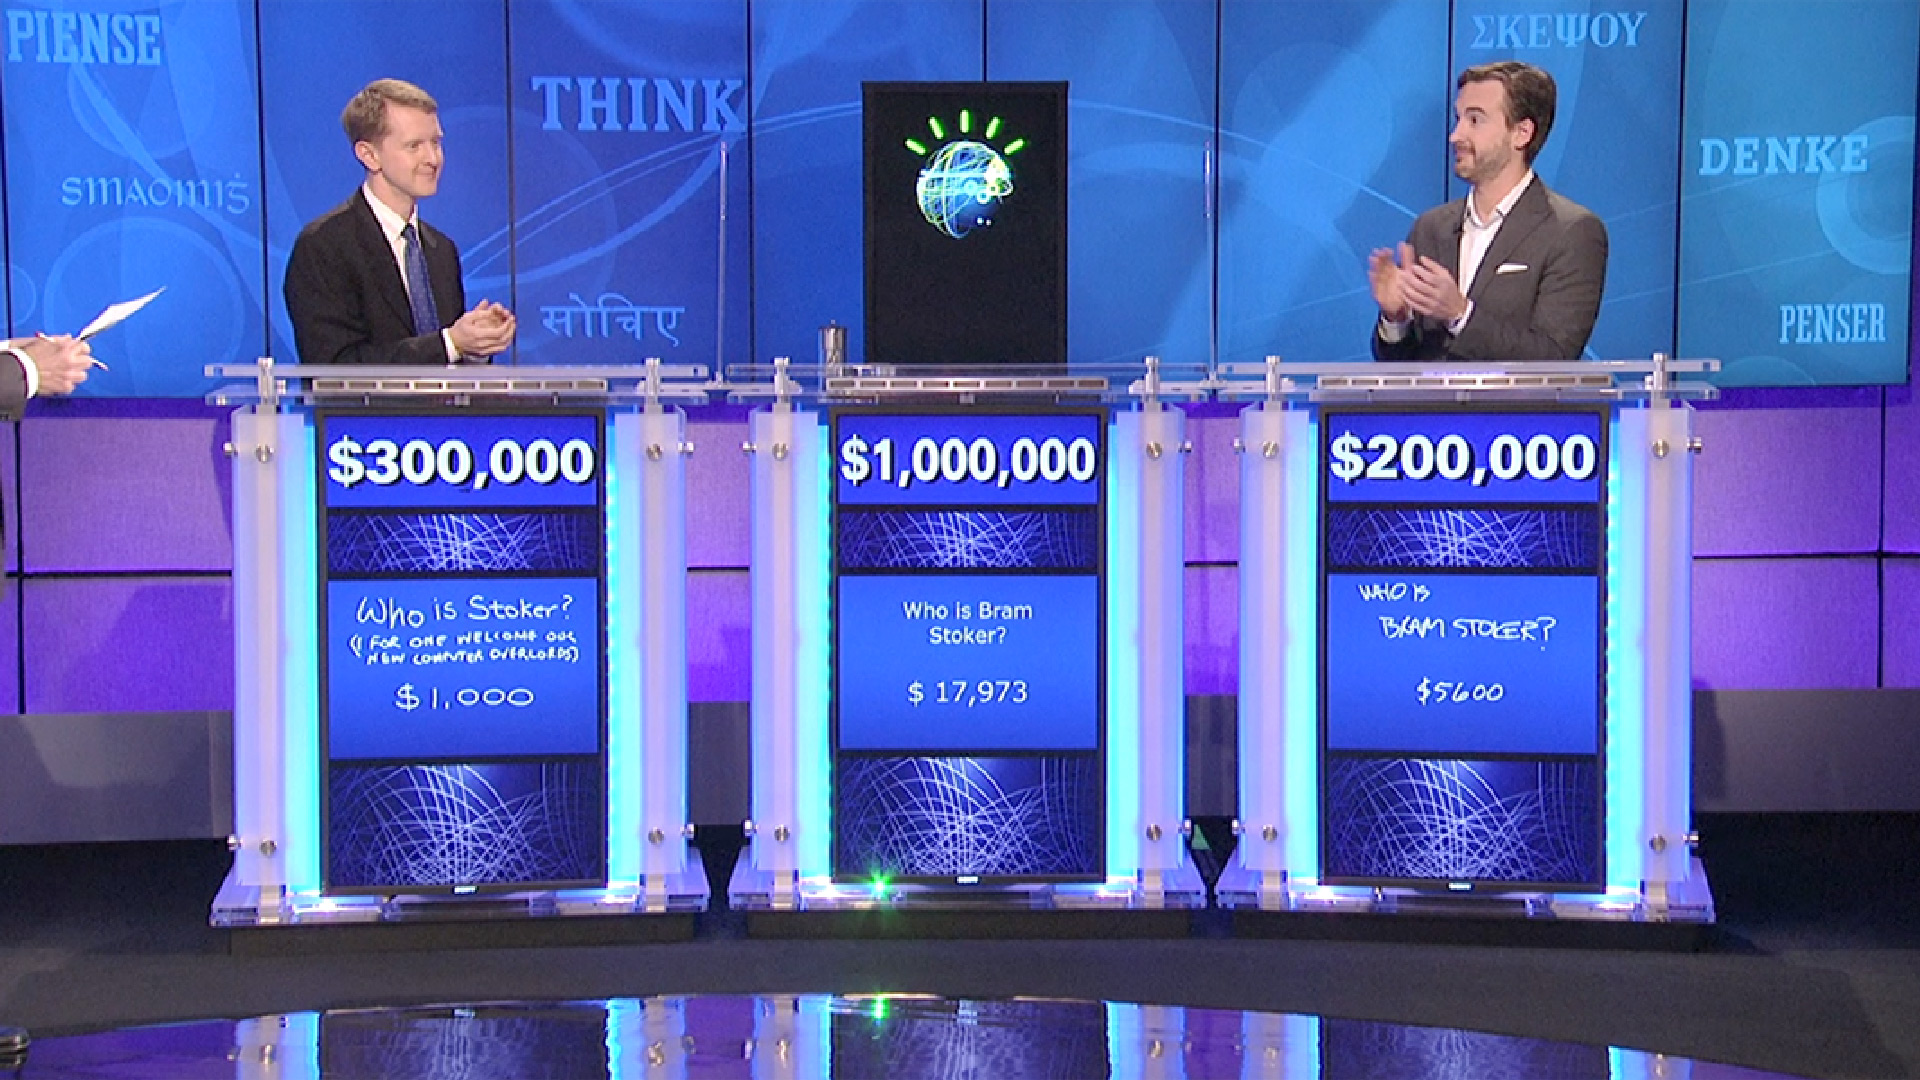
\includegraphics[width=1.0\linewidth]{qb/jeopardy}
                \pause
                \vspace{-8cm}
         \begin{block}{This is {\bf not} Jeopardy}
		\begin{itemize}
                        \item Jeopardy: must decide to answer {\bf once}, after
                          complete question
                        \item Quiz Bowl: decide after each word
		\end{itemize}

	\end{block}

\end{frame}




% TODO add more questions here

\begin{frame}[t]
	\frametitle{Sample Question}

        The Swiss-Italian architect Pietro Antonio Solari
        \only<2->{built several fortified towers in this city, which
          often vied for power with its northern rival Tver. A ruler
          of this city prevailed in the} \only<3->{Great Stand on the
          Ugra River. A prince from this city was nicknamed for
          winning a battle on the} \only<4->{Don river. Partly because
          a ruler of this city married} \only<5->{Sophia Palaiologina,
          the niece of the last Byzantine Emperor, this city styled
          itself the} \only<6->{``Third Rome'' after the fall of
          Constantinople. Another prince of this city stopped paying
          tribute to the} \only<7->{Mongols in 1476, ending the
          ``Tatar yoke.''} \only<8->{The Grand Duchy headquartered in
          this city came to an end in 1547 with the ascension of}
        \only<9->{ Ivan IV, who made it his capital. For 10 points,
          name this city where Ivan III renovated the
          Kremlin,} \only<10->{the capital of Russia.}\\
        \vspace{.5cm} \only<11->{ {\bf Moscow} (Moskva / Muscovy)}



\end{frame}





\begin{frame}{}

  \begin{columns}
    \column{.4\linewidth}
        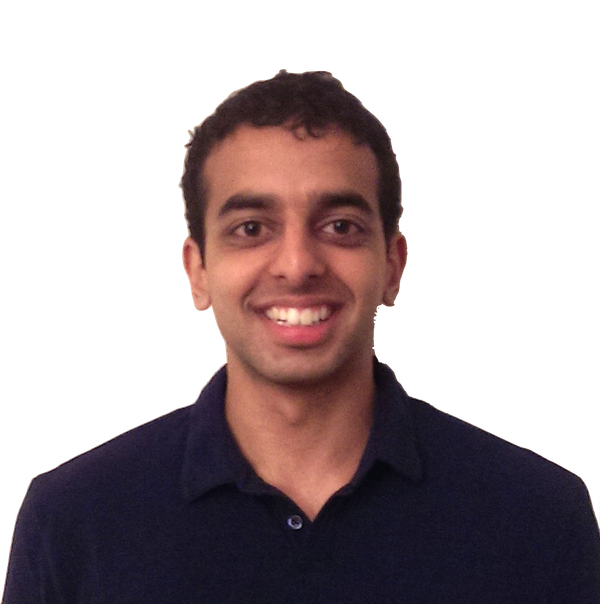
\includegraphics[width=0.7\linewidth]{general_figures/mohit}
    \column{.6\linewidth}
        \begin{block}{ {\bf \href{http://umiacs.umd.edu/~jbg//docs/2014_emnlp_qb_rnn.pdf}{A Neural Network for Factoid Question Answering over Paragraphs}}}
\underline{\href{http://cs.umd.edu/~miyyer/}{Mohit Iyyer}}, {\bf Jordan Boyd-Graber}, Leonardo Claudino, Richard Socher, and Hal {Daum\'{e} III}.  \emph{Empirical Methods in Natural Language Processing}, 2014
        \end{block}

        \begin{block}{ {\bf \href{file:///Users/jbg/public_html/docs/2015_acl_dan.pdf}{Deep Unordered Composition Rivals Syntactic Methods for Text Classification}}}
\underline{\href{http://cs.umd.edu/~miyyer/}{Mohit Iyyer}}, Varun
Manjunatha, {\bf Jordan Boyd-Graber} and Hal {Daum\'{e} III}.  \emph{Empirical Methods in Natural Language Processing}, 2014
        \end{block}

  \end{columns}
\end{frame}


\begin{frame}{Experiment 1}

		\begin{columns}
			\column{.25\linewidth}
				\gfxq{colby_jeo}{1.0}
                                Colby Burnett:
                                \$375,000
			\column{.25\linewidth}
				\gfxq{ben_jeo}{1.0}
                                Ben Ingram:
                                \$427,534
			\column{.25\linewidth}
				\gfxq{alex_jeo}{1.0}
                                Alex Jacobs: \$151,802
			\column{.25\linewidth}
				\gfxq{kristin_jeo}{1.0}
                                Kristin Sausville: \$95,201
		\end{columns}

                \pause


                \begin{center}
                End result: 200-200 tie!
                \end{center}

\end{frame}

\fsi{qb/hsnct1}{}
\fsi{qb/nasat}{Humans 345-145}
\fsi{qb/hsnct_2017}{Computer 260-215}


\begin{frame}[plain]
\gfxq{seattle_crowd}{.5}
\gfxq{chicago_crowd}{.5}
\end{frame}

\fsi{qb/boring_dot_products}{}

\fsi{simtrans/centaur-chess}{Centaur Chess}


\fsi{qb/augment/screenshot_all}{Interface}

\fsi{qb/augment/screenshot_guesses}{}

\fsi{qb/augment/screenshot_highlight}{{\bf Highlighting}}

\fsi{qb/augment/screenshot_evidence}{}

\begin{frame}{Experts vs. Novices}

 \begin{block}{Experts}
   Trivia experts, familiar with task, enjoy the task
 \end{block}

 \begin{block}{Mechanical Turkers}
   Mechanical Turkers: easily overwhelmed, need the help
 \end{block}

\end{frame}

\fsi{qb/augment/tools_acc}{Evidence helps novices, experts are expert}
\fsi{qb/augment/tools_buzz}{Hights help experts}

\begin{frame}{Regression Analysis}
    For each triple (player, question, interpretations), we predict the outcome
    (correct answer or not) with a logistic regression. The features include:
    \begin{itemize}
        \item player ID
        \item question ID
        \item buzzing position
        \item enabled interpretations: individual and combinations
    \end{itemize}

    \pause

    \begin{block}{Coefficients tell story!}
      \begin{itemize}
        \item {\bf Big, Positive}: Help
        \item {\bf Big, Negative}: Hurt
        \item {\bf Small}: Neutral
      \end{itemize}
    \end{block}

\end{frame}


\fsi{qb/augment/coefs_0}{Everything helps: Evidence for novies,
  Highlight for experts}
\fsi{qb/augment/coefs_1}{Synergistic effects}
\fsi{qb/augment/coefs_2}{Highlight and evidence help experts most}
\fsi{qb/augment/coefs_3}{For novices, less synergy}


\begin{frame}{}

  \begin{columns}
    \column{.4\linewidth}
    \begin{center}
        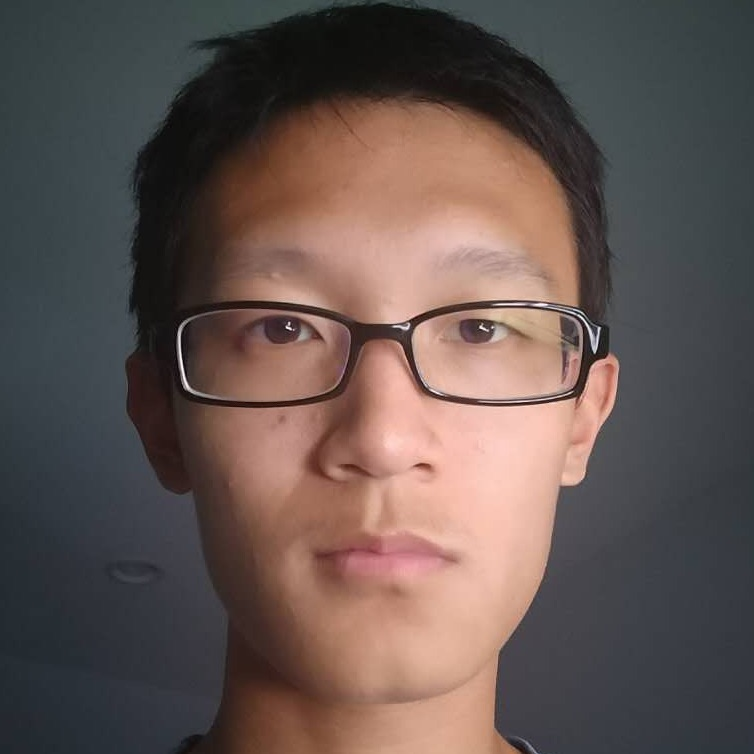
\includegraphics[width=0.8\linewidth]{general_figures/shi}
        \end{center}
    \column{.6\linewidth}
    \begin{block}{\href{http://umiacs.umd.edu/~jbg//docs/2023_emnlp_augment.pdf}{Learning to Explain Selectively}}
      \underline{\href{http://users.umiacs.umd.edu/~shifeng/}{Shi Feng}} and {\bf Jordan Boyd-Graber}.  \emph{Empirical Methods in Natural Language Processing}, 2022
        \end{block}

  \end{columns}
\end{frame}


\begin{frame}{Measuring Interpretability}

  \only<1>{\gfxq{qb_centaur_1}{.9}}
  \only<2>{\gfxq{qb_centaur_2}{.9}}
  \only<3>{\gfxq{qb_centaur_3}{.9}}
  \only<4>{\gfxq{qb_centaur_6}{.9}}

\end{frame}


\begin{frame}{Improvement through Reinforcement Learning}

  \only<1>{\gfxq{rl_centaur_2}{.9}}
  \only<2>{\gfxq{rl_centaur_3}{.9}}
  \only<3>{\gfxq{rl_centaur_4}{.9}}
  \only<4>{\gfxq{rl_centaur_5}{.9}}
  \only<5>{\gfxq{rl_centaur_6}{.9}}

\end{frame}


\fsi{qb/augment/bandit_result}{Personalization after forty questions}

\begin{frame}{}
  \begin{columns}
    \column{.2\linewidth}
    \begin{center}
        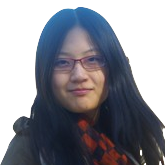
\includegraphics[width=0.8\linewidth]{general_figures/hehe} \\
        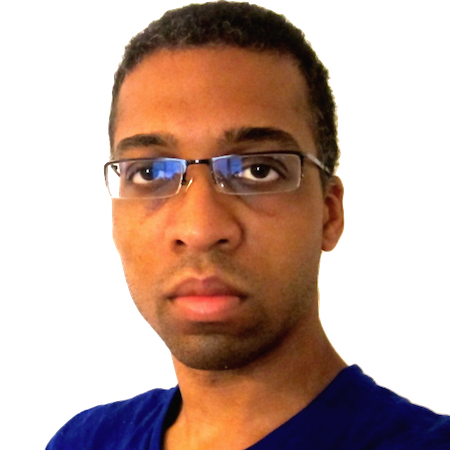
\includegraphics[width=0.8\linewidth]{general_figures/alvin}
        \\
        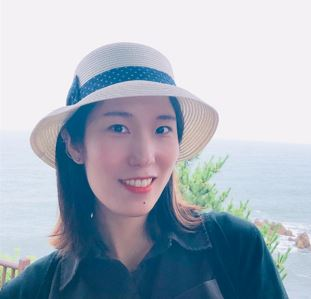
\includegraphics[width=0.8\linewidth]{general_figures/hyojung}
        \end{center}
    \column{.8\linewidth}

        \begin{block}{ {\bf
              \href{http://umiacs.umd.edu/~jbg//docs/2015_emnlp_rewrite.pdf}{Syntax-based
                Rewriting for Simultaneous Machine Translation}}}
          \small
He He, Alvin Grissom II, {\bf Jordan Boyd-Graber}, and Hal {Daum\'{e} III}.  \emph{Empirical Methods in Natural Language Processing}, 2015
        \end{block}

        \begin{block}{ {\bf
              \href{http://umiacs.umd.edu/~jbg/docs/2016_naacl_interpretese.pdf}{Interpretese
                vs. Translationese: The Uniqueness of Human Strategies
                in Simultaneous Interpretation}}}
          \small
He He, {\bf Jordan Boyd-Graber}, and Hal {Daum\'{e} III}.
\emph{North American Association for Computational Linguistics}, 2016
        \end{block}


        \begin{block}{ {\bf
              \href{http://umiacs.umd.edu/~jbg/docs/2022_emnlp_simint.pdf}{SimQA:
                Detecting Simultaneous MT Errors through 
                Word-by-Word Question Answering}}}
          \small
          \href{https://h-j-han.github.io/}{HyoJung Han}, Marine
            Carpuat, {\bf Jordan Boyd-Graber}.  \emph{Empirical Methods in Natural Language Processing}, 2022
          
          \end{block}
  \end{columns}


\end{frame}

\begin{frame}{Simultaneous Interpretation is Hard!}

  \begin{columns}
    \column{.5\linewidth}
  \begin{itemize}
    \item Exhausting for humans
    \item Computers not trusted
    \item Differential strengths
    \item Same word-by-word characteristic
  \end{itemize}

  \column{.5\linewidth}
 \gfxs{computer-interpreter}{1.0}
 \end{columns}
\end{frame}

\begin{frame}{Undertranslation}
  \begin{center}
    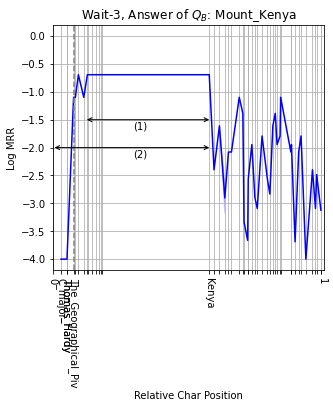
\includegraphics[width=0.5\paperwidth]{simtrans/simQA/ex_undertranslation}
  \end{center}
When the information doesn't
help an answerer, it's not producing anything useful
\end{frame}

\begin{frame}{Undertranslation}
  \begin{center}
    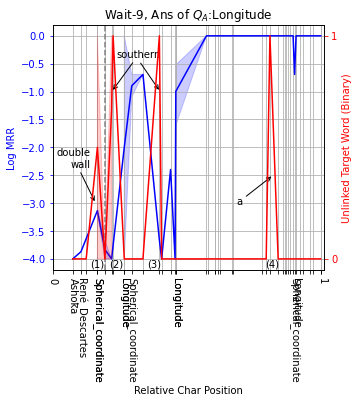
\includegraphics[width=0.5\paperwidth]{simtrans/simQA/ex_hallucination}
  \end{center}
When the information confuses an
  answerer, it's actively hindering!
\end{frame}


\begin{frame}

\makebox[\linewidth]{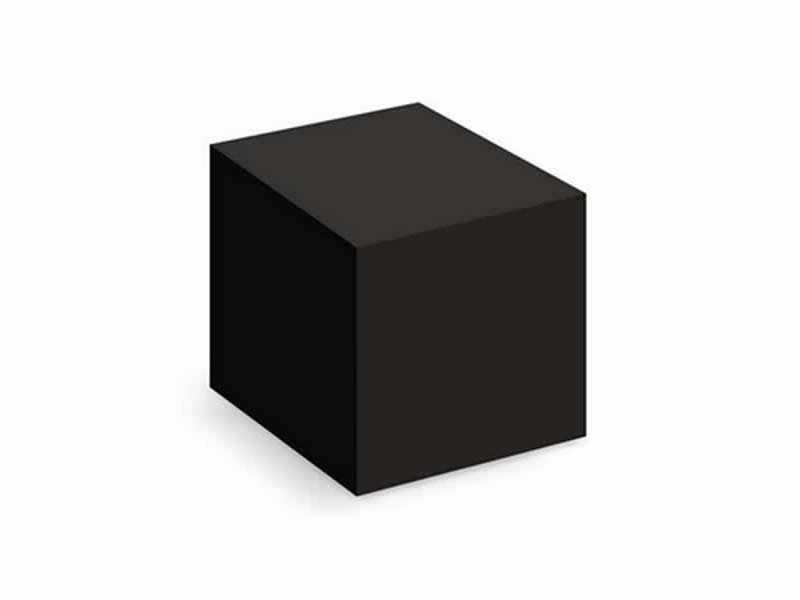
\includegraphics[width=\paperwidth]{general_figures/blackbox}}
\only<2>{

\vspace{-5cm}
\begin{block}{Takeaways}
  \begin{itemize}
    \item ML should be interpretable
    \item We should measure interpretability
    \item Interpretability should reflect the world we want
  \end{itemize}
\end{block}

}
\end{frame}


\frame{

	\frametitle{Thanks}

        \begin{block}{Collaborators}
          \textsc{naqt}, Hal Daum\'e III (UMD), Marine Carpuat, Leah Findlater (UMD), Kevin Seppi
          (BYU), Eric Ringger
        \end{block}

	\begin{columns}

	\column{.75\linewidth}
        \begin{block}{Funders}
        \begin{center}
          
\includegraphics[width=0.2\linewidth]{general_figures/nsf}
          
\includegraphics[width=0.2\linewidth]{general_figures/darpa}
          
\includegraphics[width=0.2\linewidth]{general_figures/arl}
          
\includegraphics[width=0.2\linewidth]{general_figures/iarpa}
       \end{center}
        \end{block}

	\column{.3\linewidth}
        \begin{block}{Supporters}
        	\gfxq{naqt}{1.0}
        \end{block}

        \end{columns}
}



\frame{

\begin{columns}

\column{.5\linewidth}

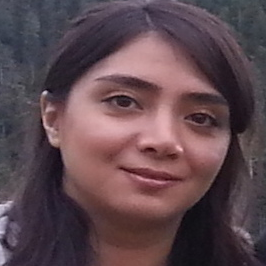
\includegraphics[width=.8\linewidth]{general_figures/forough}

\column{.5\linewidth}

\begin{block}{ALTO: Active Learning with Topic Overviews for Speeding Label Induction and Document Labeling}
Forough Poursabzi-Sangdeh, Jordan Boyd-Graber, Leah Findlater, and Kevin Seppi.  Association for Computational Linguistics, 2016.
\end{block}

\end{columns}

}



\fsi{interactive_topic_models/alto_interface}{}
\fsi{interactive_topic_models/alto_interface_highlight}{Direct users
  to document}



\fsi{interactive_topic_models/alto/user_talk_1}{ Active learning if time is short}
\fsi{interactive_topic_models/alto/user_talk_2}{ Better than status quo}
\fsi{interactive_topic_models/alto/user_talk_3}{ Active learning can
  help topic models }
\fsi{interactive_topic_models/alto/user_talk_4}{ Topic models help
  users understand the collection }
\fsi{interactive_topic_models/alto/user_talk_4}{ Moral: machines and
  humans together (if you let them) }


\fsi{qb/viz_first_draft}{Andrea Lin}


\begin{frame}{References}
\bibliographystyle{style/acl}
\tiny
\bibliography{bib/journal-full,bib/jbg,bib/hhe,bib/alvin,teaparty/vietan,bib/hoyle}
\end{frame}



\begin{frame}{RC TRUST}
\begin{center}
  
\includegraphics[width=0.7\paperwidth]{job_talks/trust_research_centers}
\end{center}
\small
  \only<2>{
    \begin{columns}
      \column{.6\linewidth}
    \begin{block}{Psychology \& Social Sciences}
      \begin{itemize}
      \item Method: Item Response Theory
      \item Method: Ideal Point Models
        \item Application: Multilingual and Multicultural Models of
          Persuasion and Alliance Building
        \item Collaboration: Bundesverfassungsgericht Entscheidungen
        \end{itemize}
      \end{block}
      \column{.4\linewidth}      
      \end{columns}
  }
  
  \only<3>{
    \begin{columns}
      \column{.1\linewidth}
      \column{.6\linewidth}
      \begin{block}{AI \& ML}
              \begin{itemize}
    \item Method: Reinforcement Learning 
    \item Method: Neural Text Similarity
    \item Application: Training QA Retrieval Mechanisms
    \item Collaboration: Improving Google QA
      \end{itemize}
      \end{block}
      \column{.3\linewidth}      
    \end{columns}
  }


  \only<4>{
    \begin{columns}
      \column{.3\linewidth}
      \column{.6\linewidth}
      \begin{block}{Data Science \& Statistical Learning}
        \begin{itemize}
    \item Method: Bayesian Nonparametrics
    \item Method: Interactive Dirichlet Forest Priors
    \item Application: Sensemaking
    \item Collaboration: Monitoring Local Reseliency
      \end{itemize}
    \end{block}
            \column{.1\linewidth}
  \end{columns}

  }

  \only<5>{
    \begin{columns}
      \column{.4\linewidth}
      \column{.6\linewidth}
    \begin{block}{Cybersecurity and Privacy}
      \begin{itemize}
      \item Method: Adversarial Example Construction
      \item Method: Disinformation Gamefication
      \item Application: Fake News Detection
        \item Collaboration: Climate Fact Checking
      \end{itemize}

    \end{block}
      \end{columns}
  }

  
\end{frame}



\end{document}
